\chapter[Figures for the data-driven \ds and \dpl prompt fraction evaluation]{\texorpdfstring{Figures for the data-driven \ds and\\ \dpl prompt fraction evaluation}{Figures for the data-driven Ds+ and D+ prompt fraction evaluation}}\label{app:fpds}
In this Appendix, the results of the data-driven approach employed for estimating the \fpds and \fpdpl correction factors are reported. The description of the used methodologies and the content of the Figures can be found in Chapter~\ref{ch:corrections}.

\begin{sidewaysfigure}
    \centering
    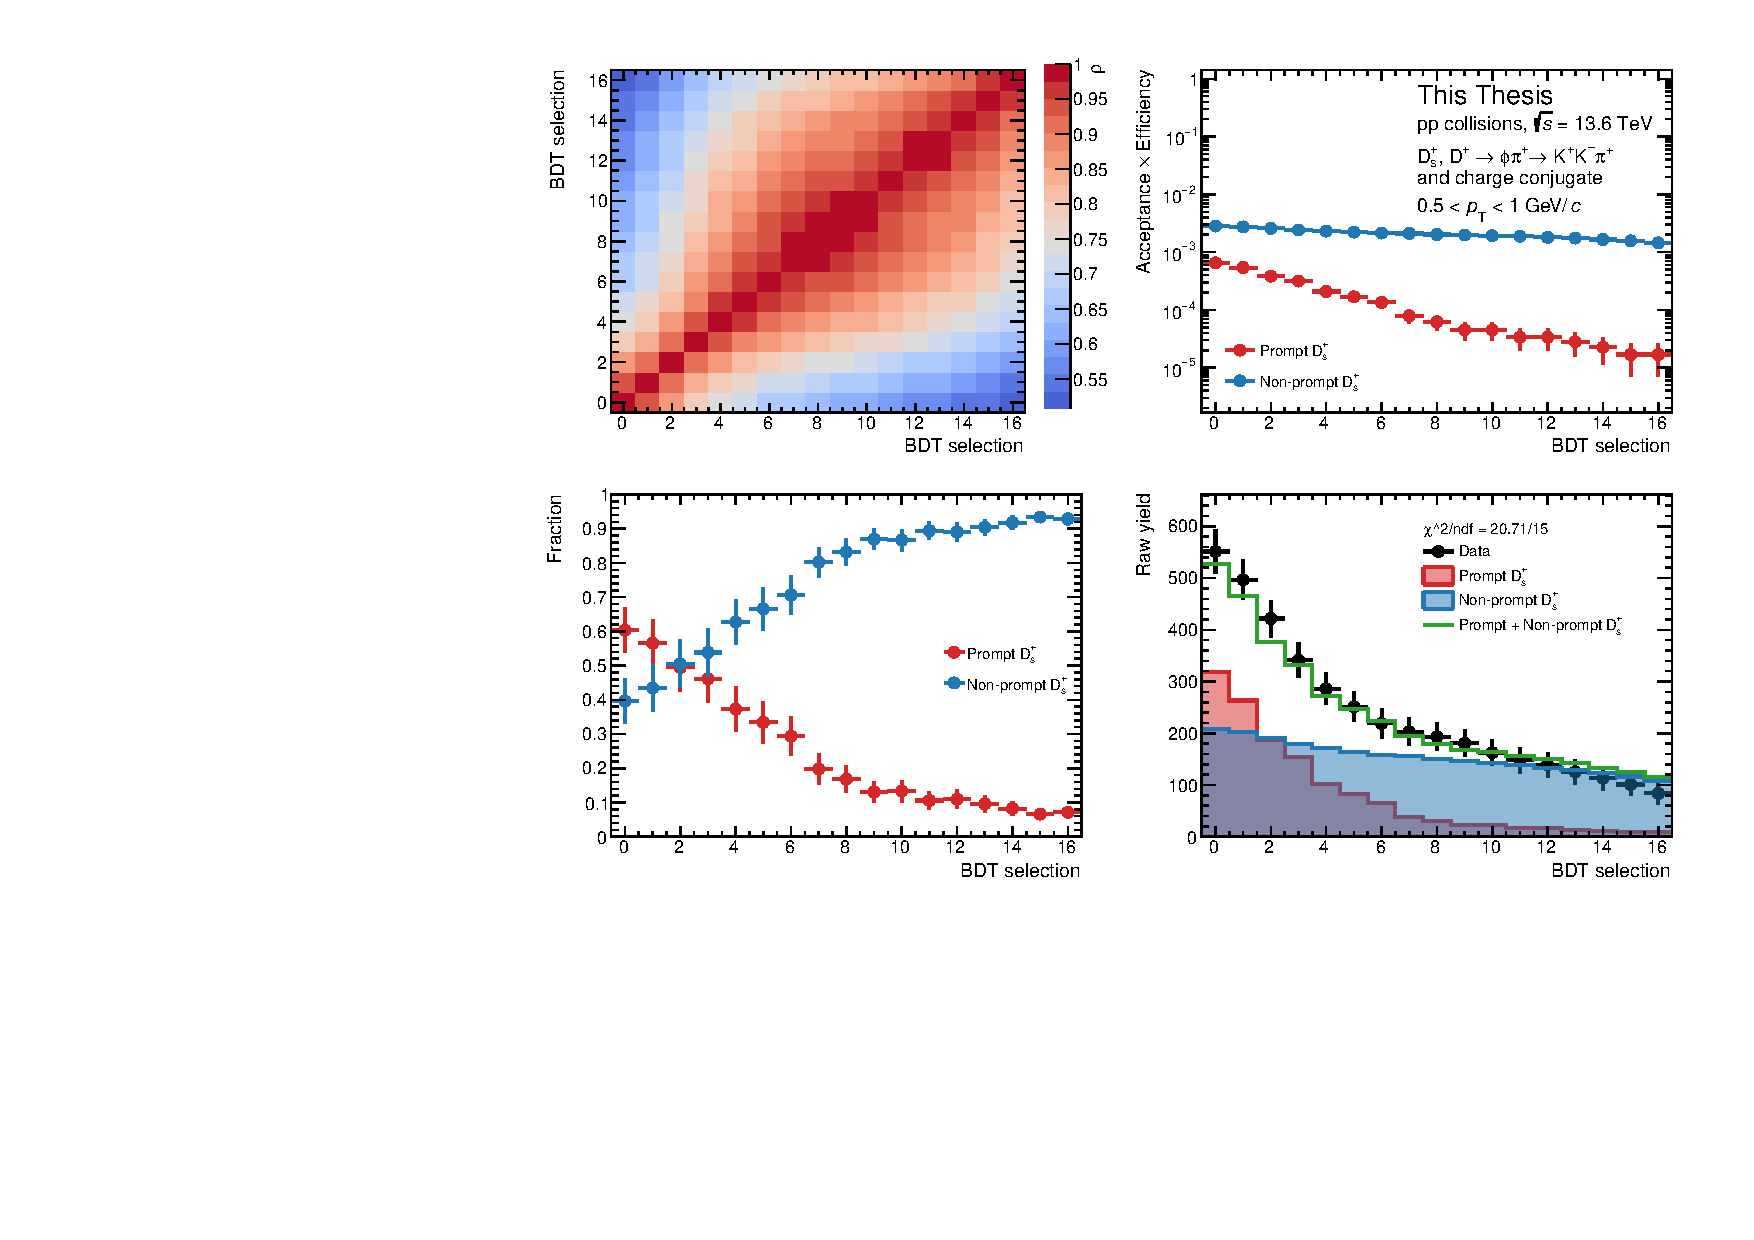
\includegraphics[width=0.48\textwidth]{Figures/Chapter 6/AllPropmtFracs/Ds/DsPromptFrac5_10.pdf}
    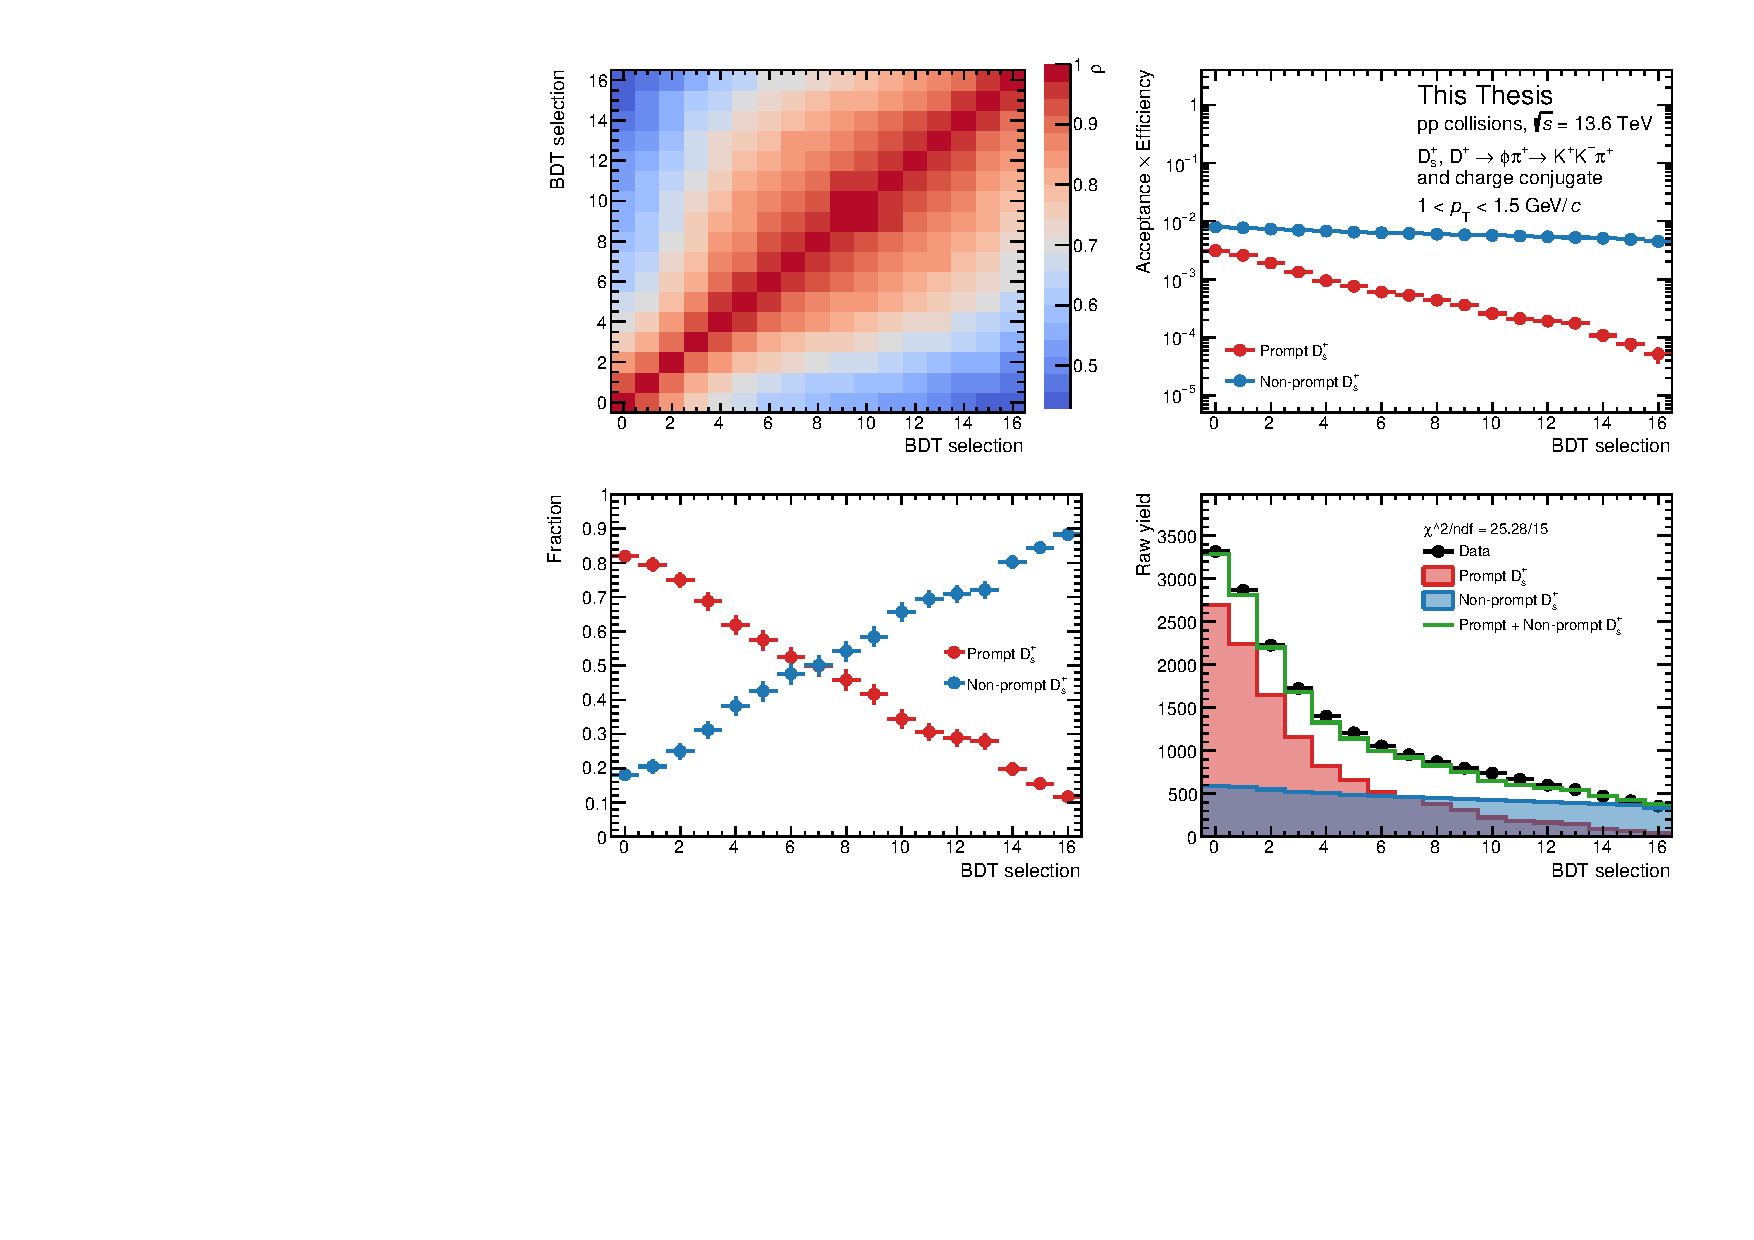
\includegraphics[width=0.48\textwidth]{Figures/Chapter 6/AllPropmtFracs/Ds/DsPromptFrac10_15.pdf}
    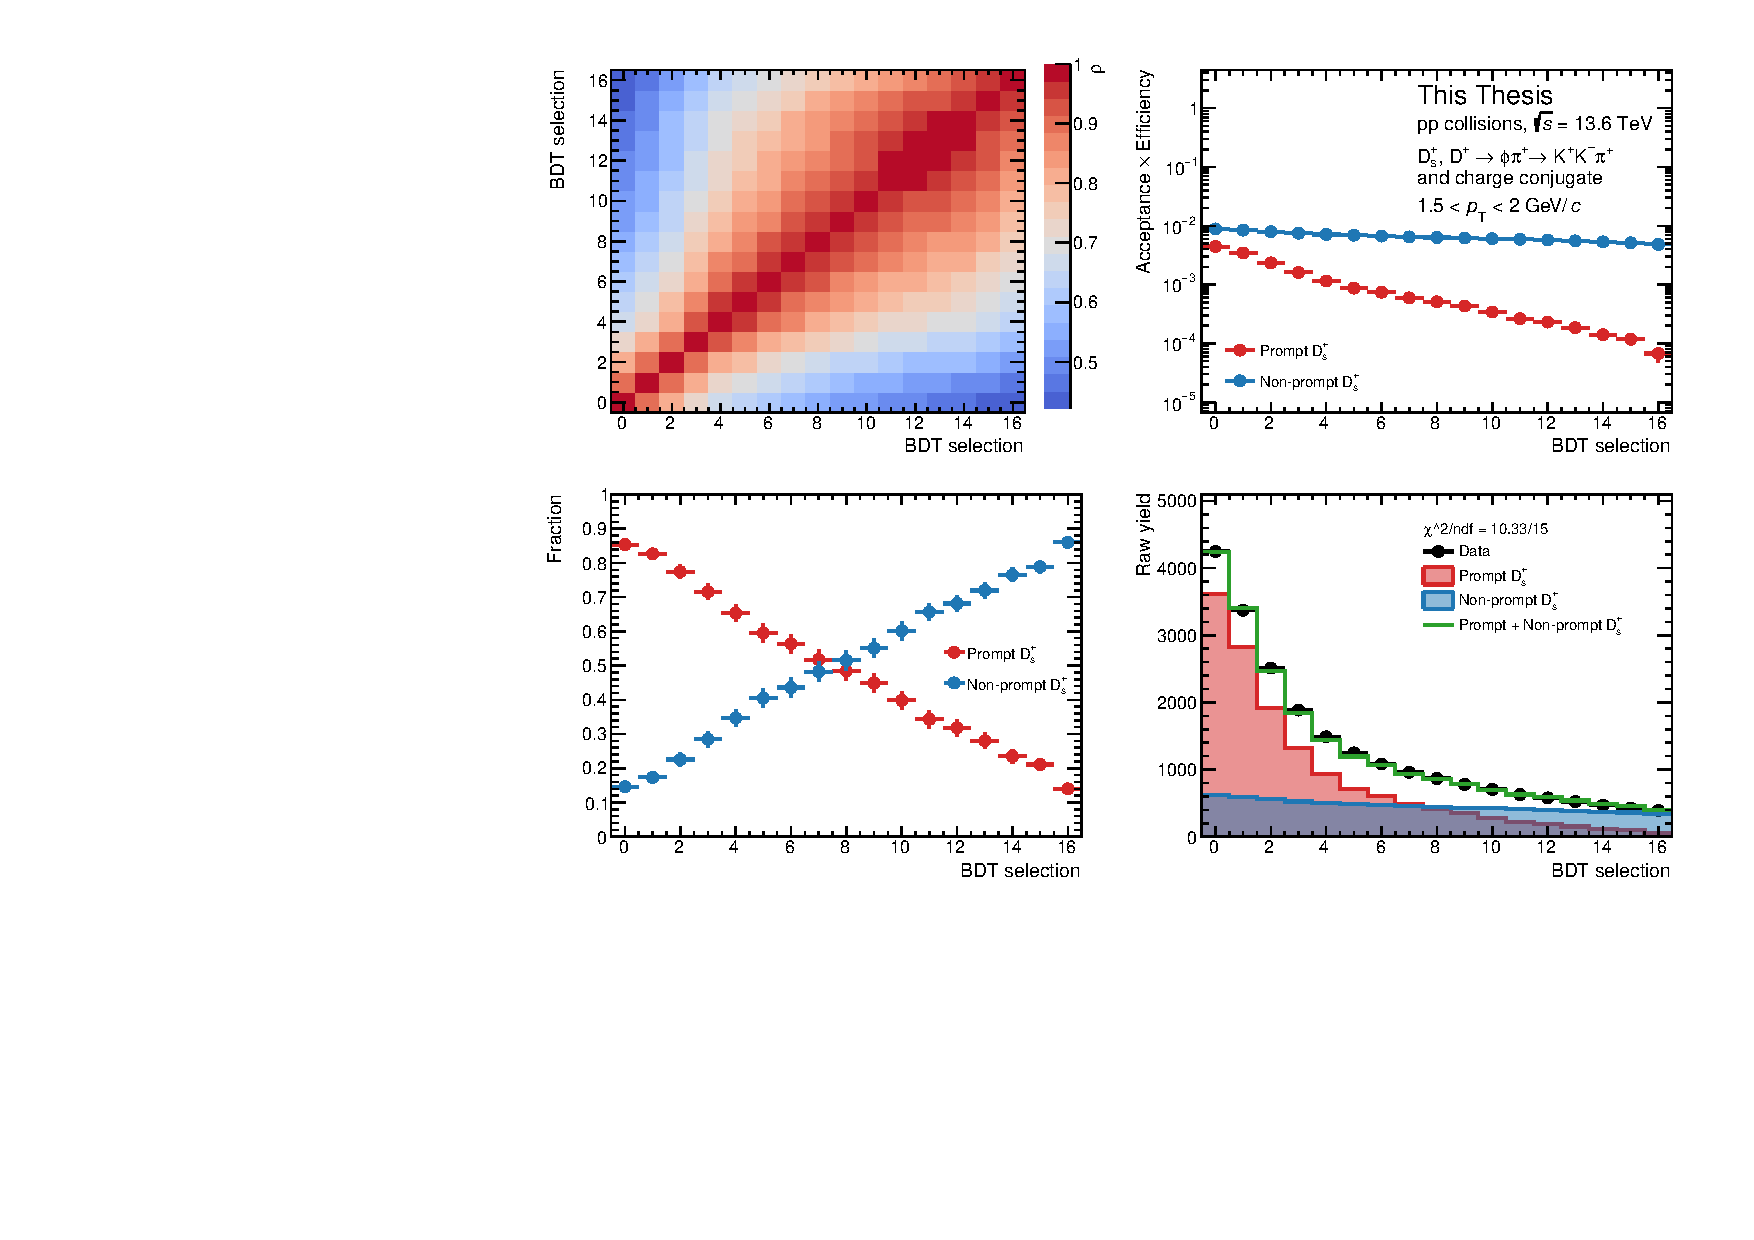
\includegraphics[width=0.48\textwidth]{Figures/Chapter 6/AllPropmtFracs/Ds/DsPromptFrac15_20.pdf}
    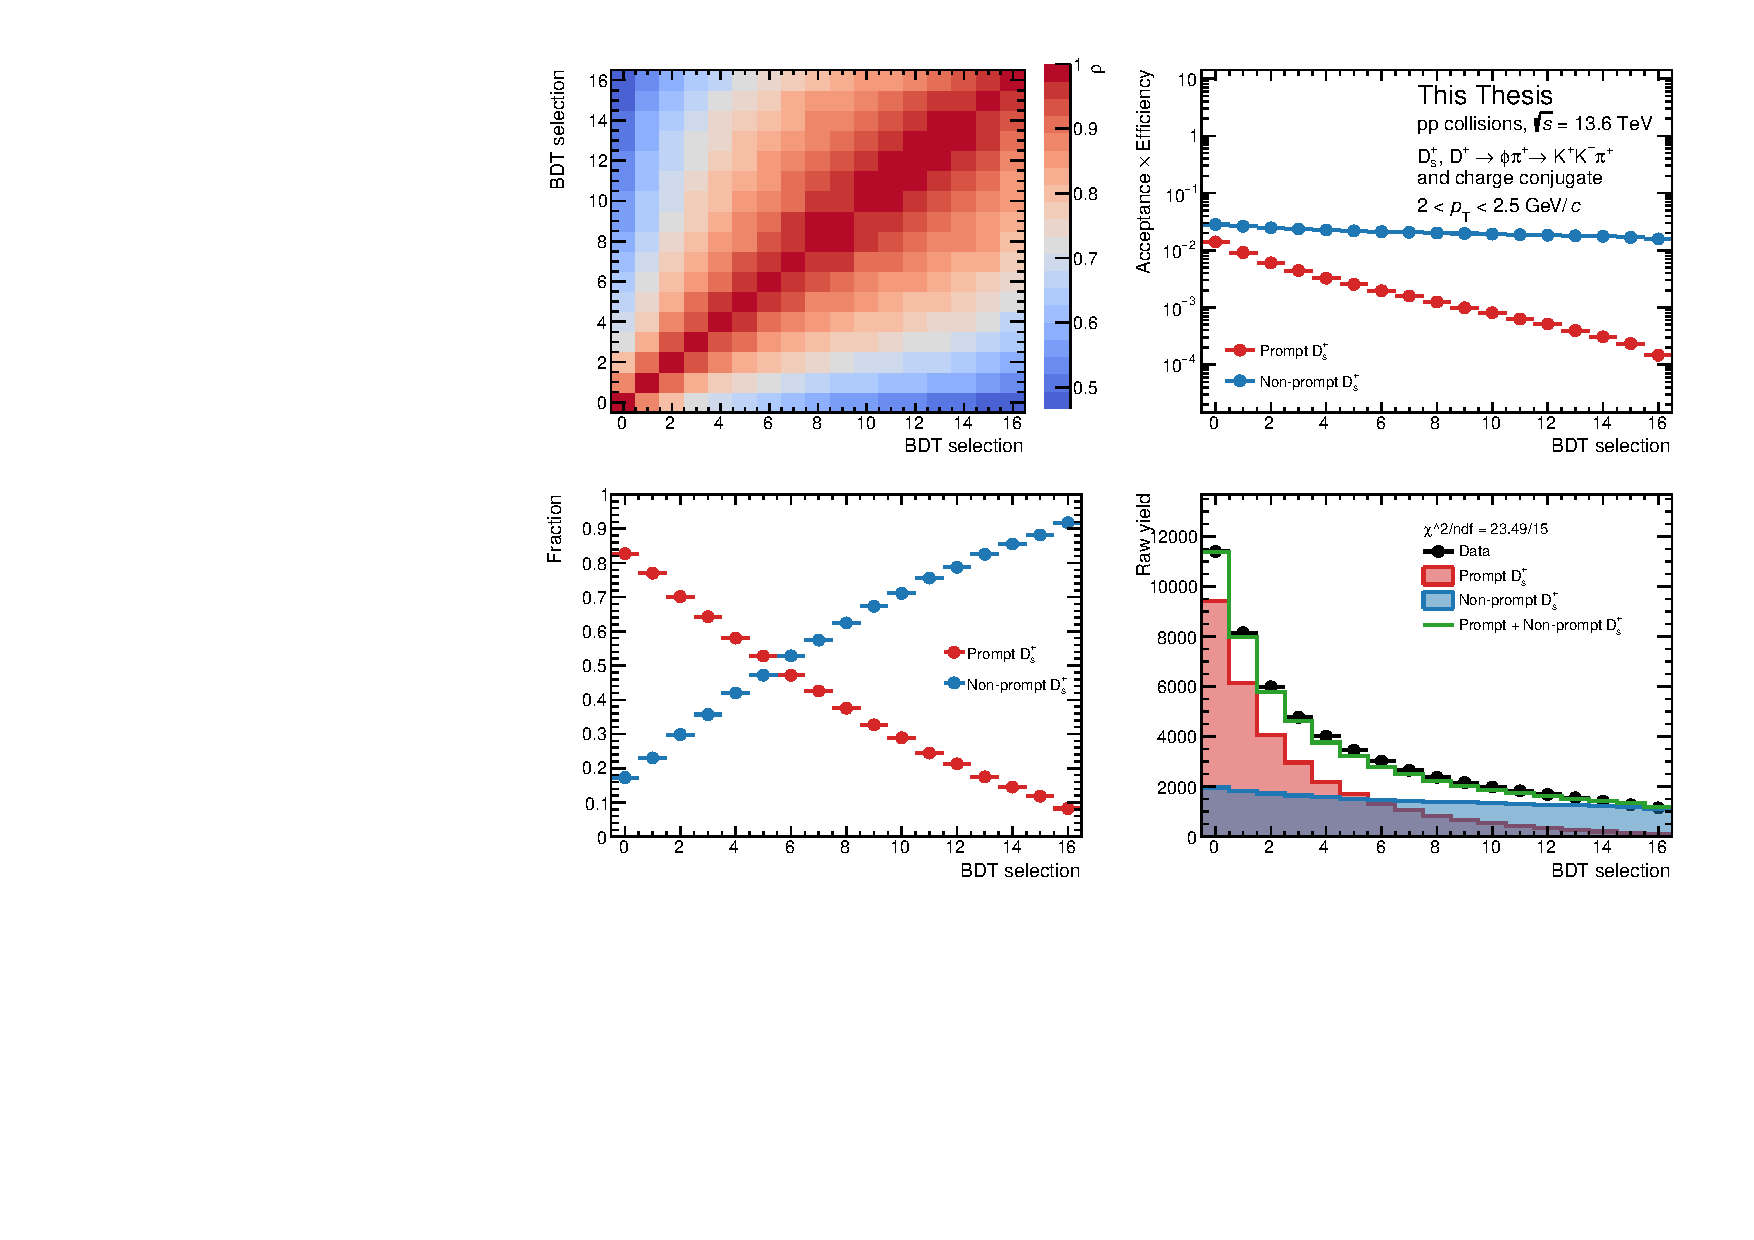
\includegraphics[width=0.48\textwidth]{Figures/Chapter 6/AllPropmtFracs/Ds/DsPromptFrac20_25.pdf}
    \caption{Results for the evaluation of the \fpds correction factor in the $0.5 < \pt < 1.0$~\gevc (top left), $1.0 < \pt < 1.5$~\gevc (top right), $1.5 < \pt < 2.0$~\gevc (bottom left) and $2.0 < \pt < 2.5$~\gevc (bottom right) intervals.}
\end{sidewaysfigure}

\begin{sidewaysfigure}
    \centering
    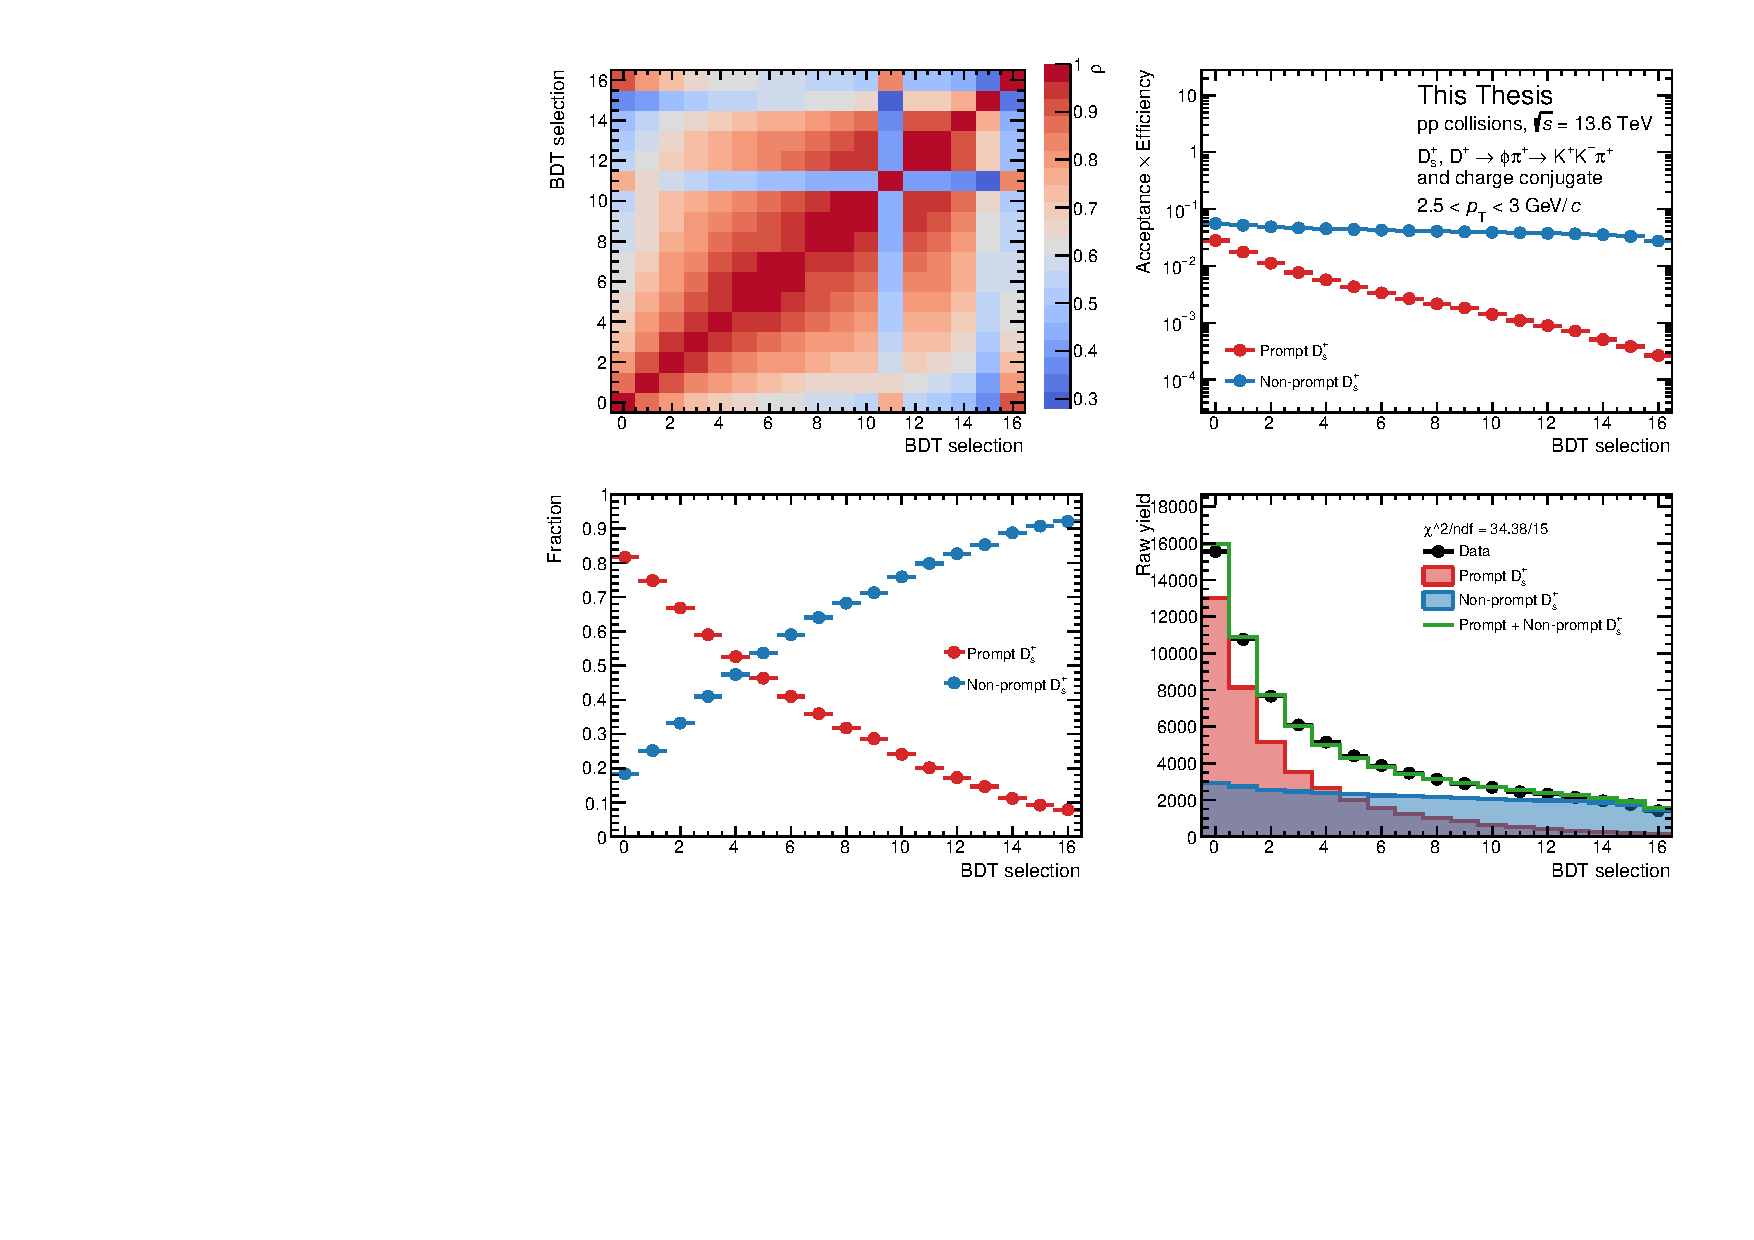
\includegraphics[width=0.48\textwidth]{Figures/Chapter 6/AllPropmtFracs/Ds/DsPromptFrac25_30.pdf}
    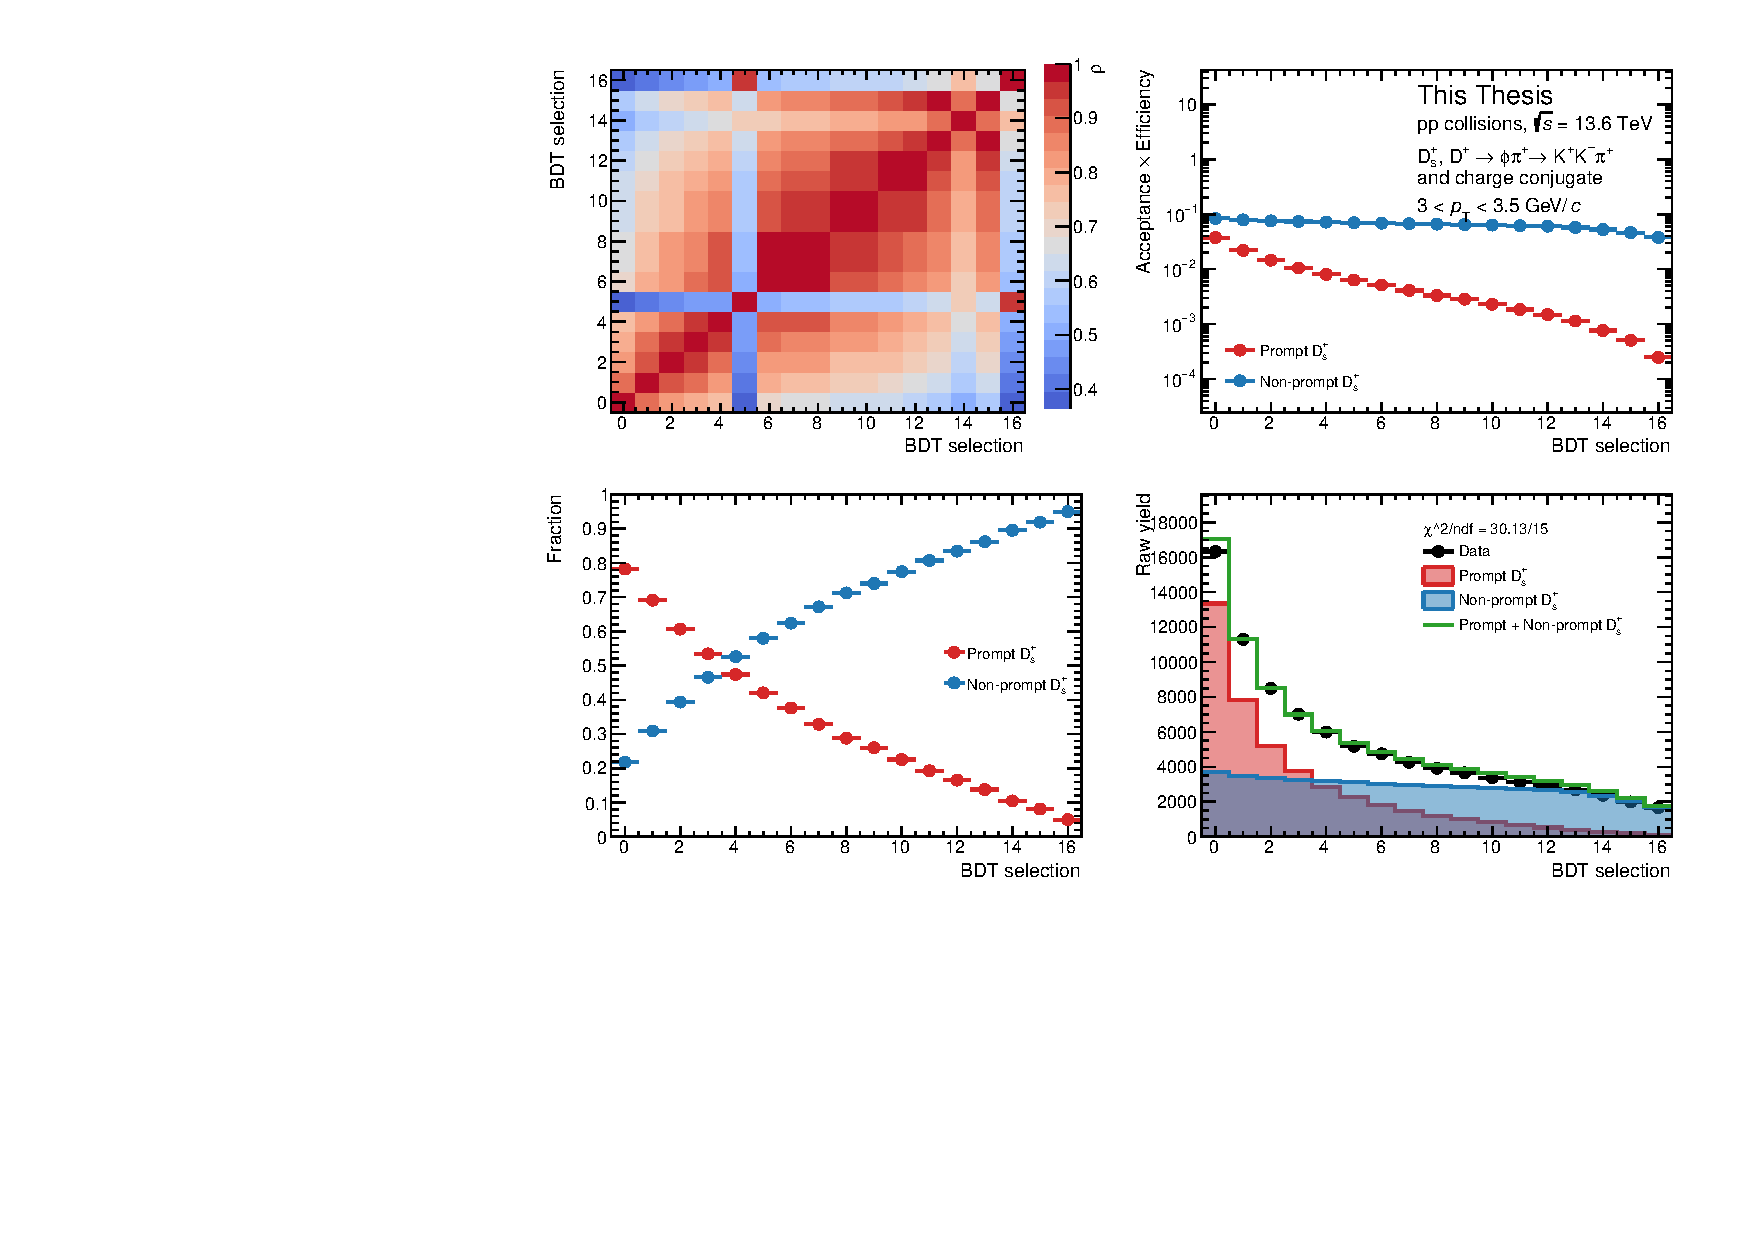
\includegraphics[width=0.48\textwidth]{Figures/Chapter 6/AllPropmtFracs/Ds/DsPromptFrac30_35.pdf}
    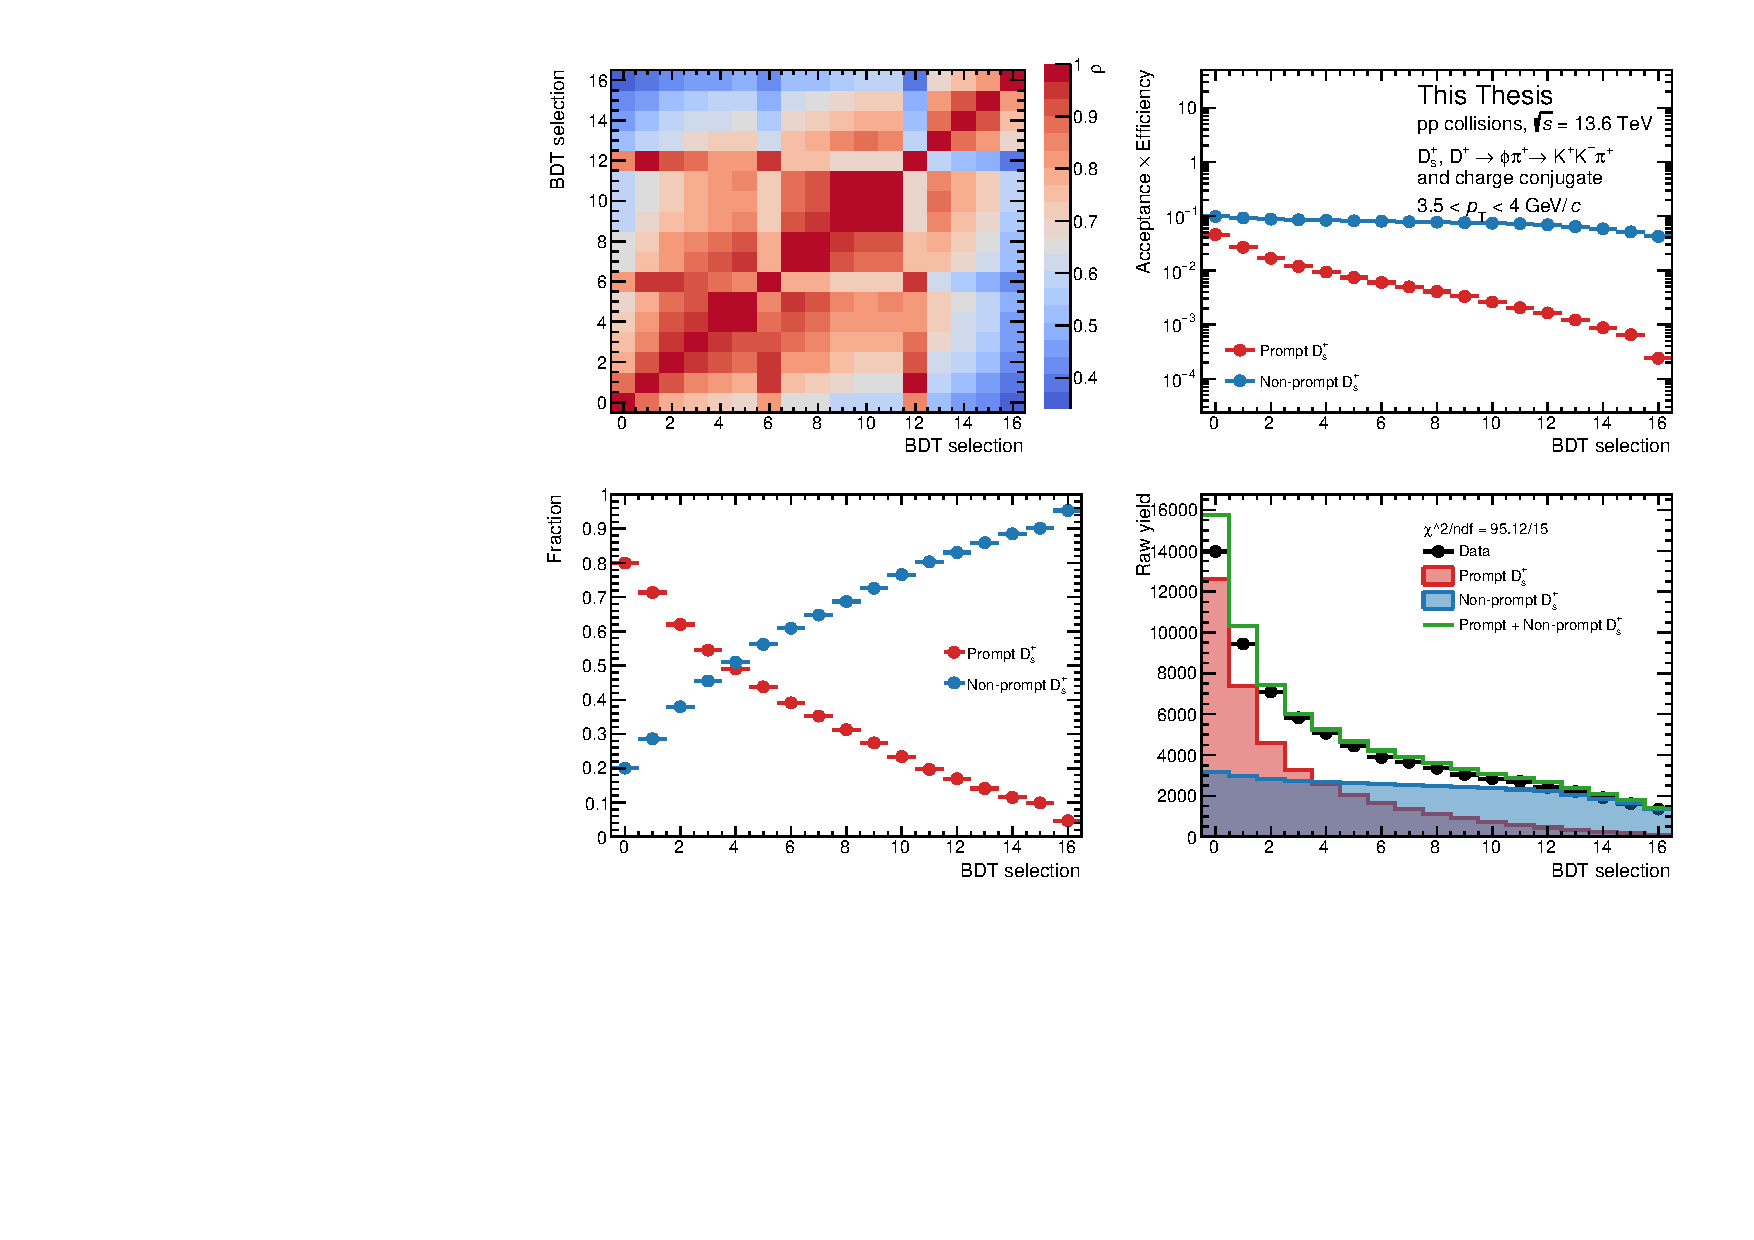
\includegraphics[width=0.48\textwidth]{Figures/Chapter 6/AllPropmtFracs/Ds/DsPromptFrac35_40.pdf}
    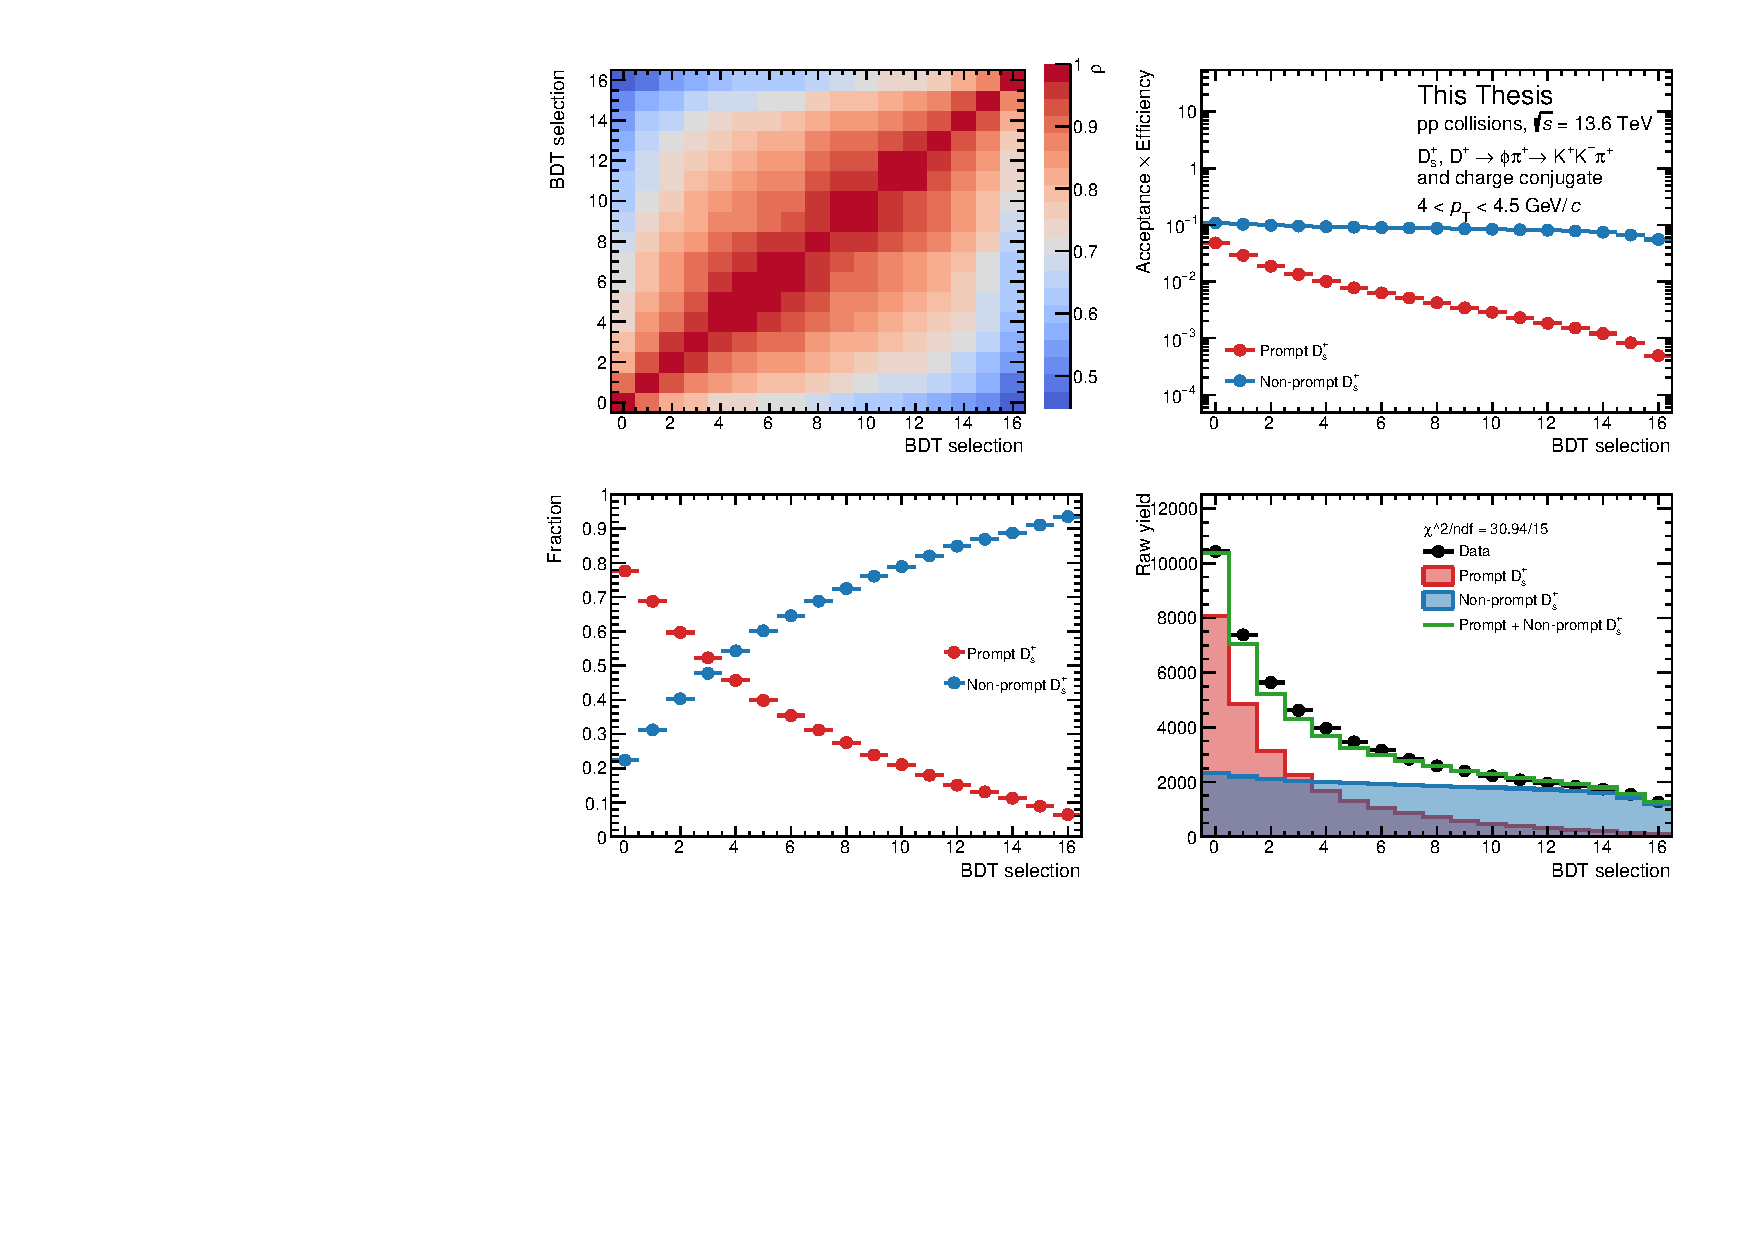
\includegraphics[width=0.48\textwidth]{Figures/Chapter 6/AllPropmtFracs/Ds/DsPromptFrac40_45.pdf}
    \caption{Results for the evaluation of the \fpds correction factor in the $2.5 < \pt < 3.0$~\gevc (top left), $3.0 < \pt < 3.5$~\gevc (top right), $3.5 < \pt < 4.0$~\gevc (bottom left) and $4.0 < \pt < 4.5$~\gevc (bottom right) intervals.}
\end{sidewaysfigure}

\begin{sidewaysfigure}
    \centering
    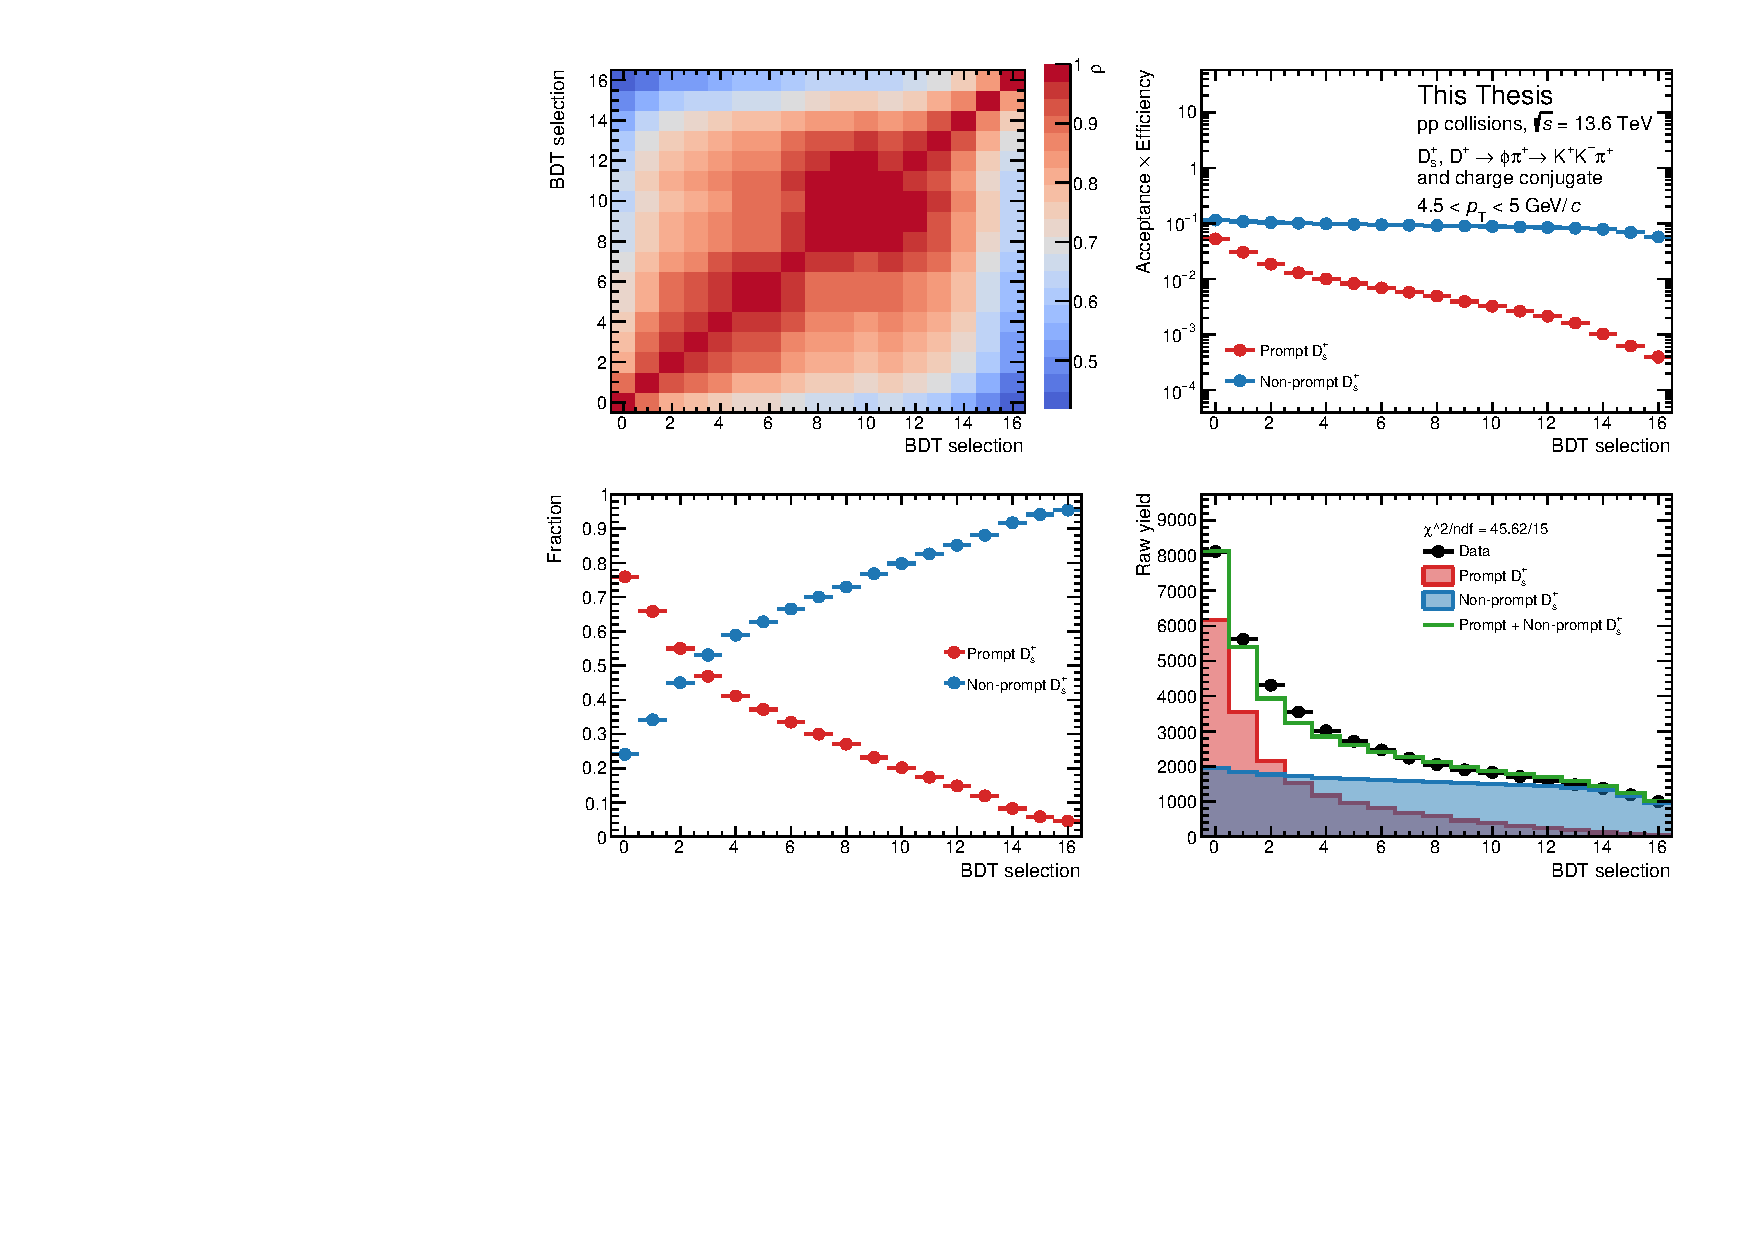
\includegraphics[width=0.48\textwidth]{Figures/Chapter 6/AllPropmtFracs/Ds/DsPromptFrac45_50.pdf}
    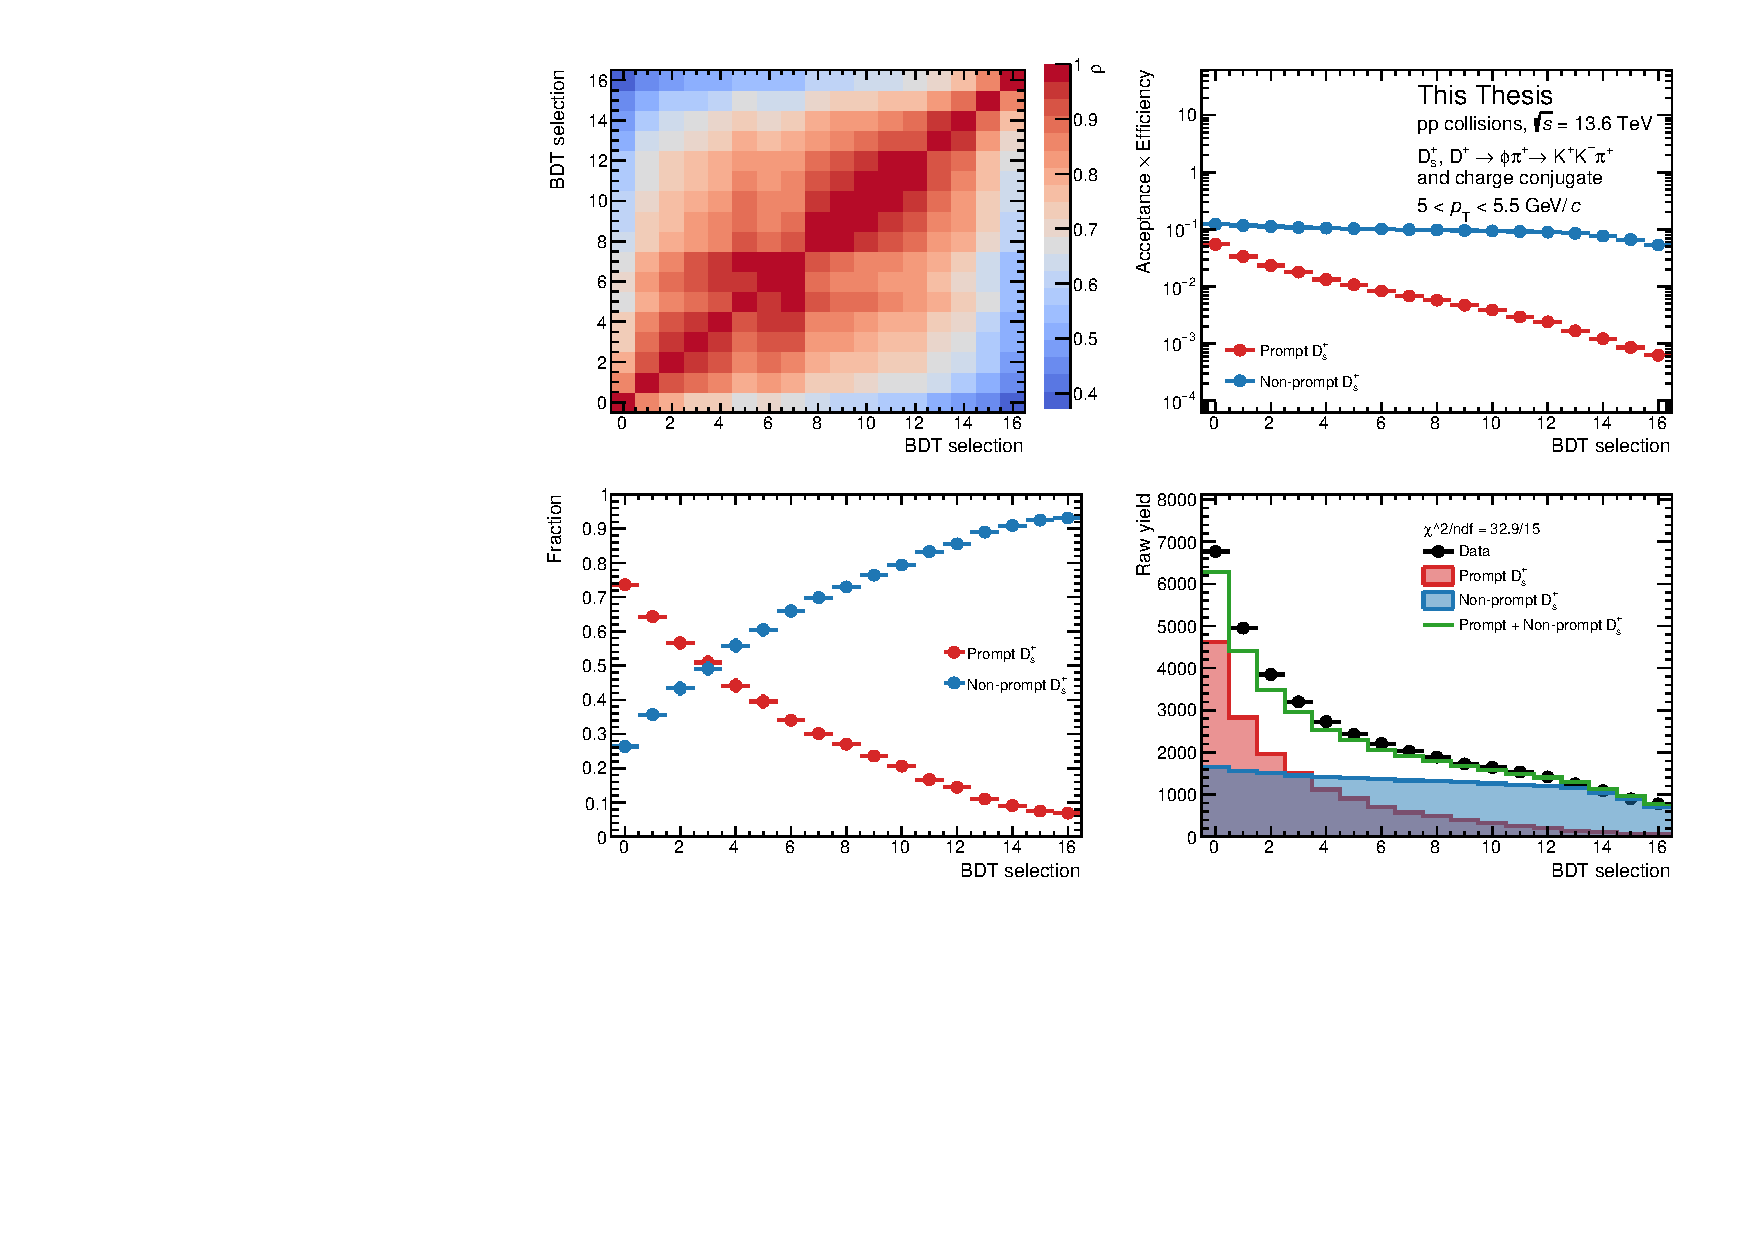
\includegraphics[width=0.48\textwidth]{Figures/Chapter 6/AllPropmtFracs/Ds/DsPromptFrac50_55.pdf}
    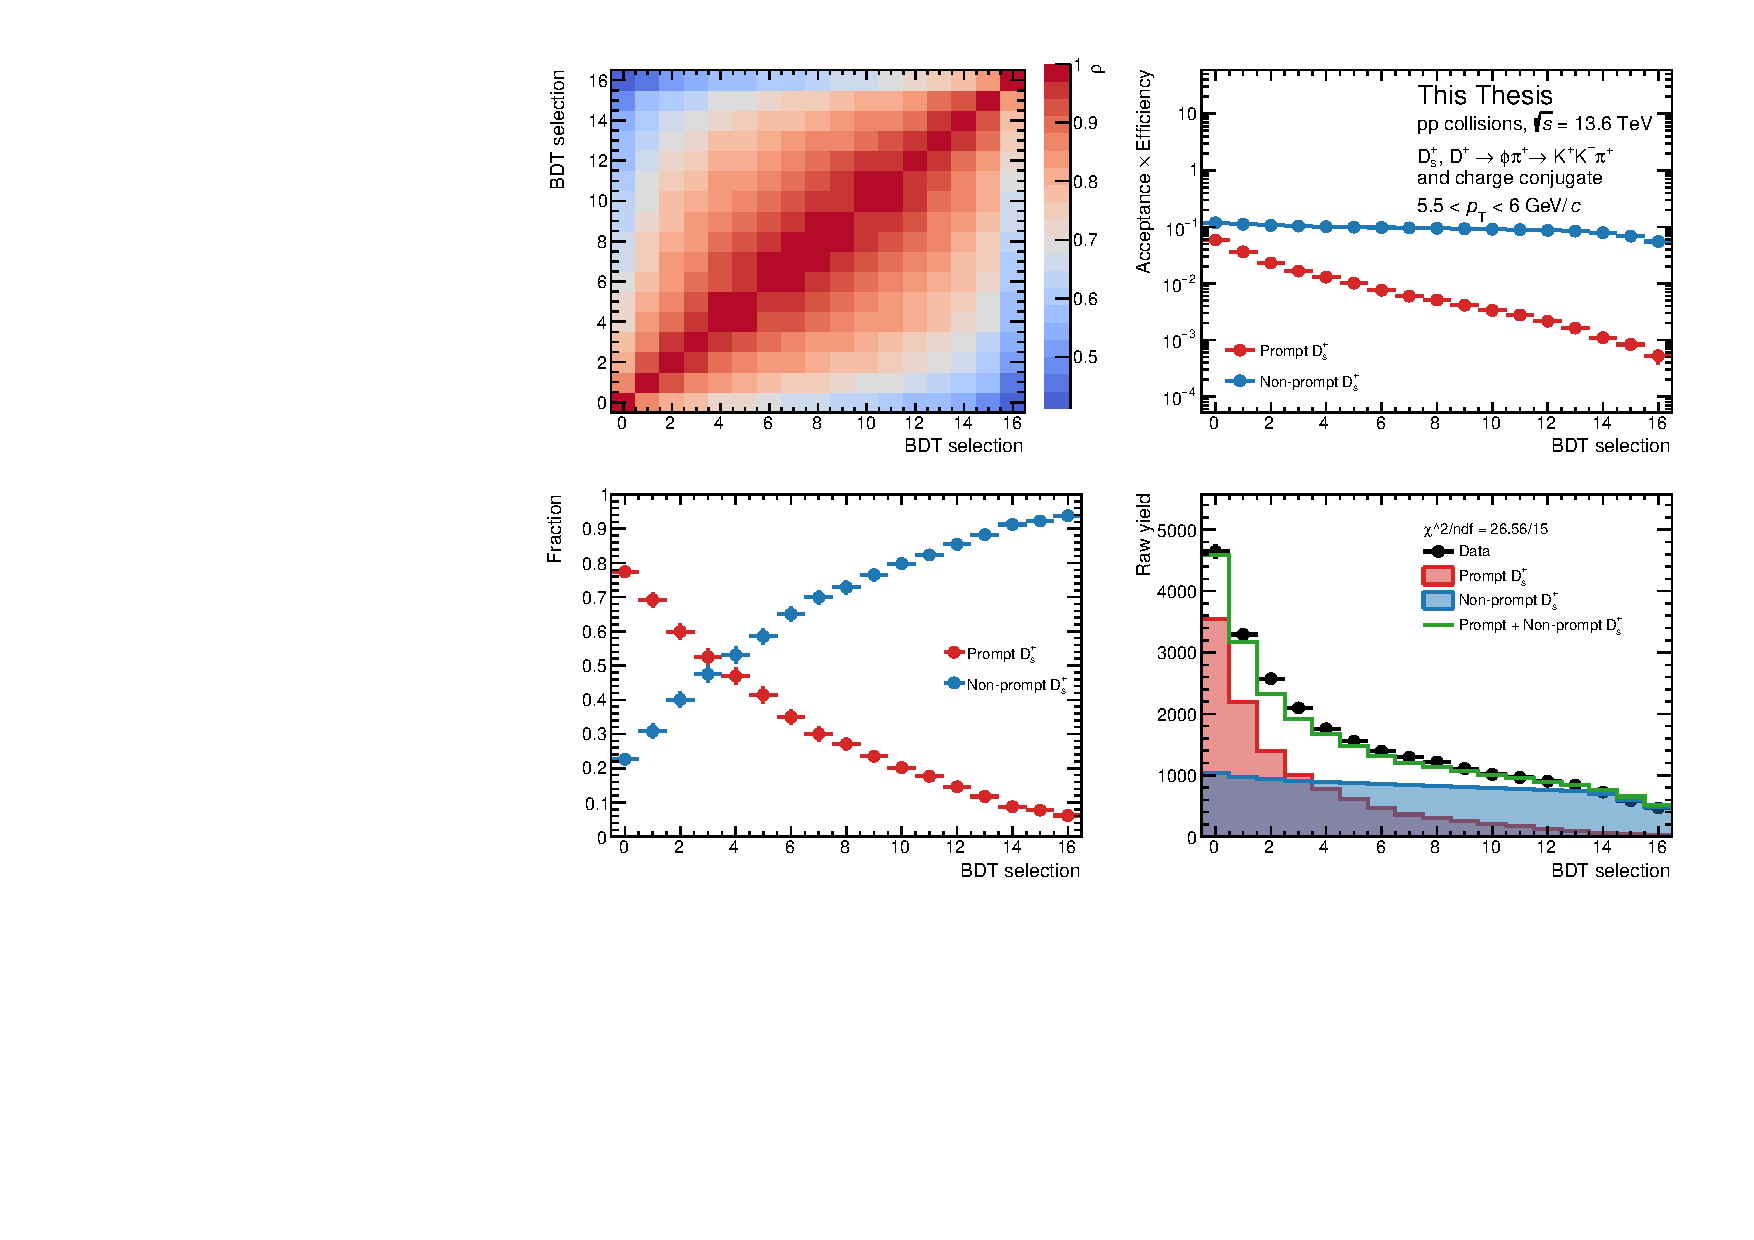
\includegraphics[width=0.48\textwidth]{Figures/Chapter 6/AllPropmtFracs/Ds/DsPromptFrac55_60.pdf}
    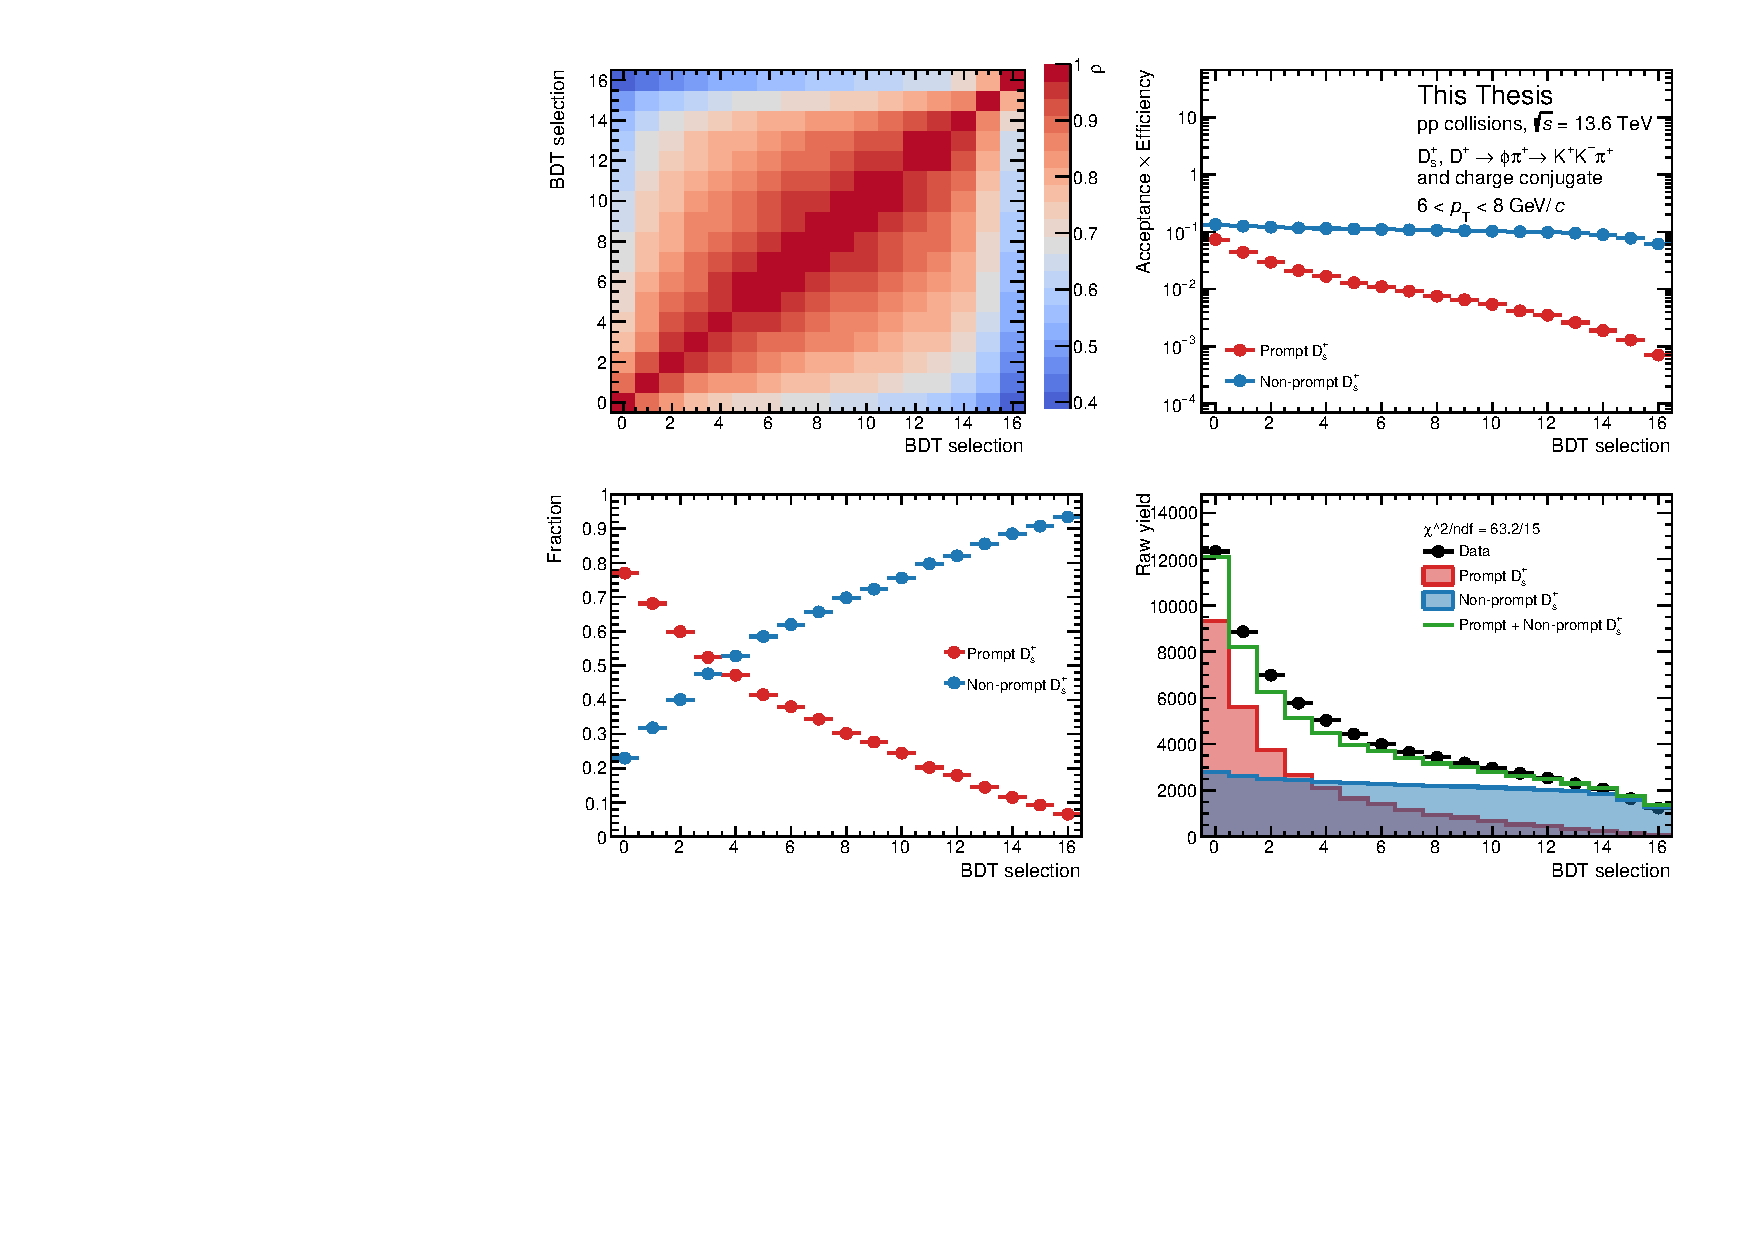
\includegraphics[width=0.48\textwidth]{Figures/Chapter 6/AllPropmtFracs/Ds/DsPromptFrac60_80.pdf}
    \caption{Results for the evaluation of the \fpds correction factor in the $4.5 < \pt < 5.0$~\gevc (top left), $5.0 < \pt < 5.5$~\gevc (top right), $5.5 < \pt < 6.0$~\gevc (bottom left) and $6.0 < \pt < 8.0$~\gevc (bottom right) intervals.}
\end{sidewaysfigure}

\begin{figure}
    \centering
    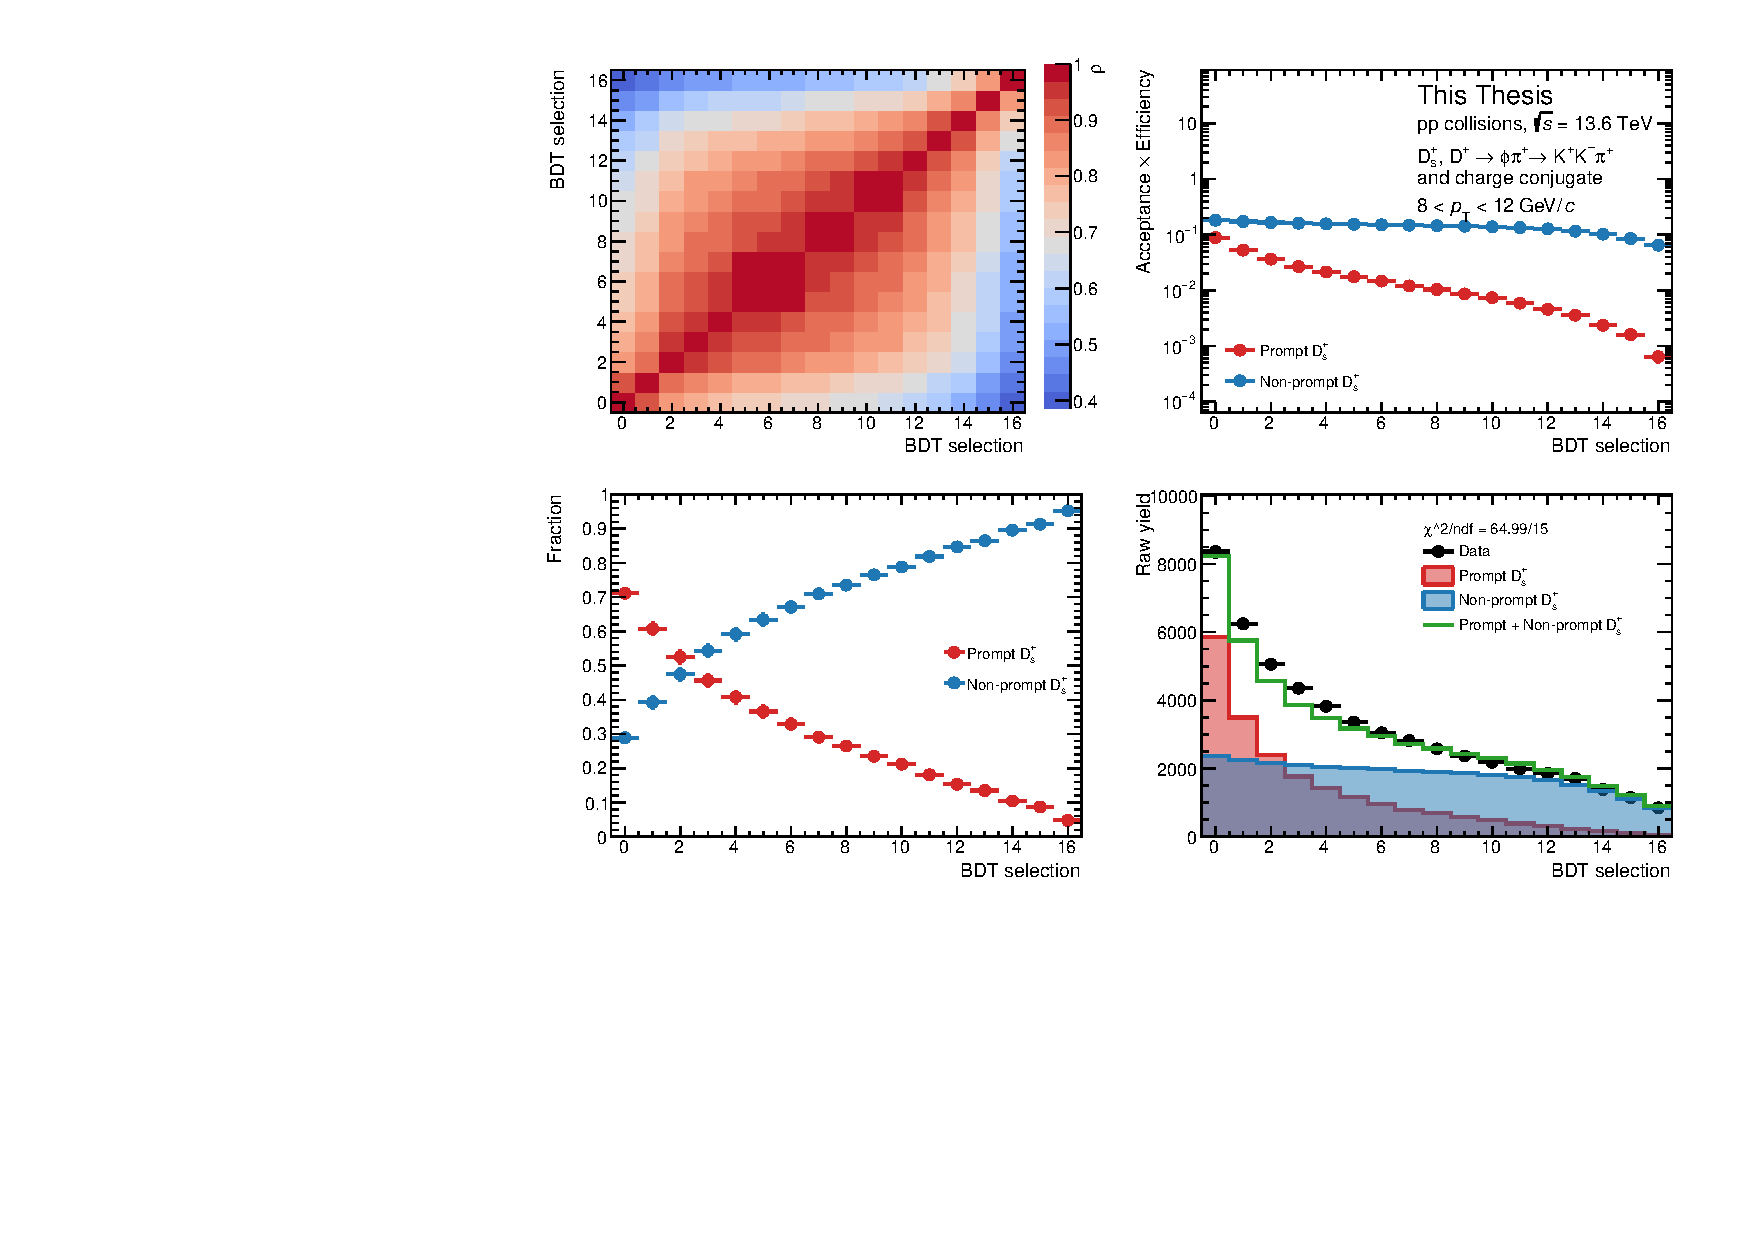
\includegraphics[width=0.7\textwidth]{Figures/Chapter 6/AllPropmtFracs/Ds/DsPromptFrac80_120.pdf}
    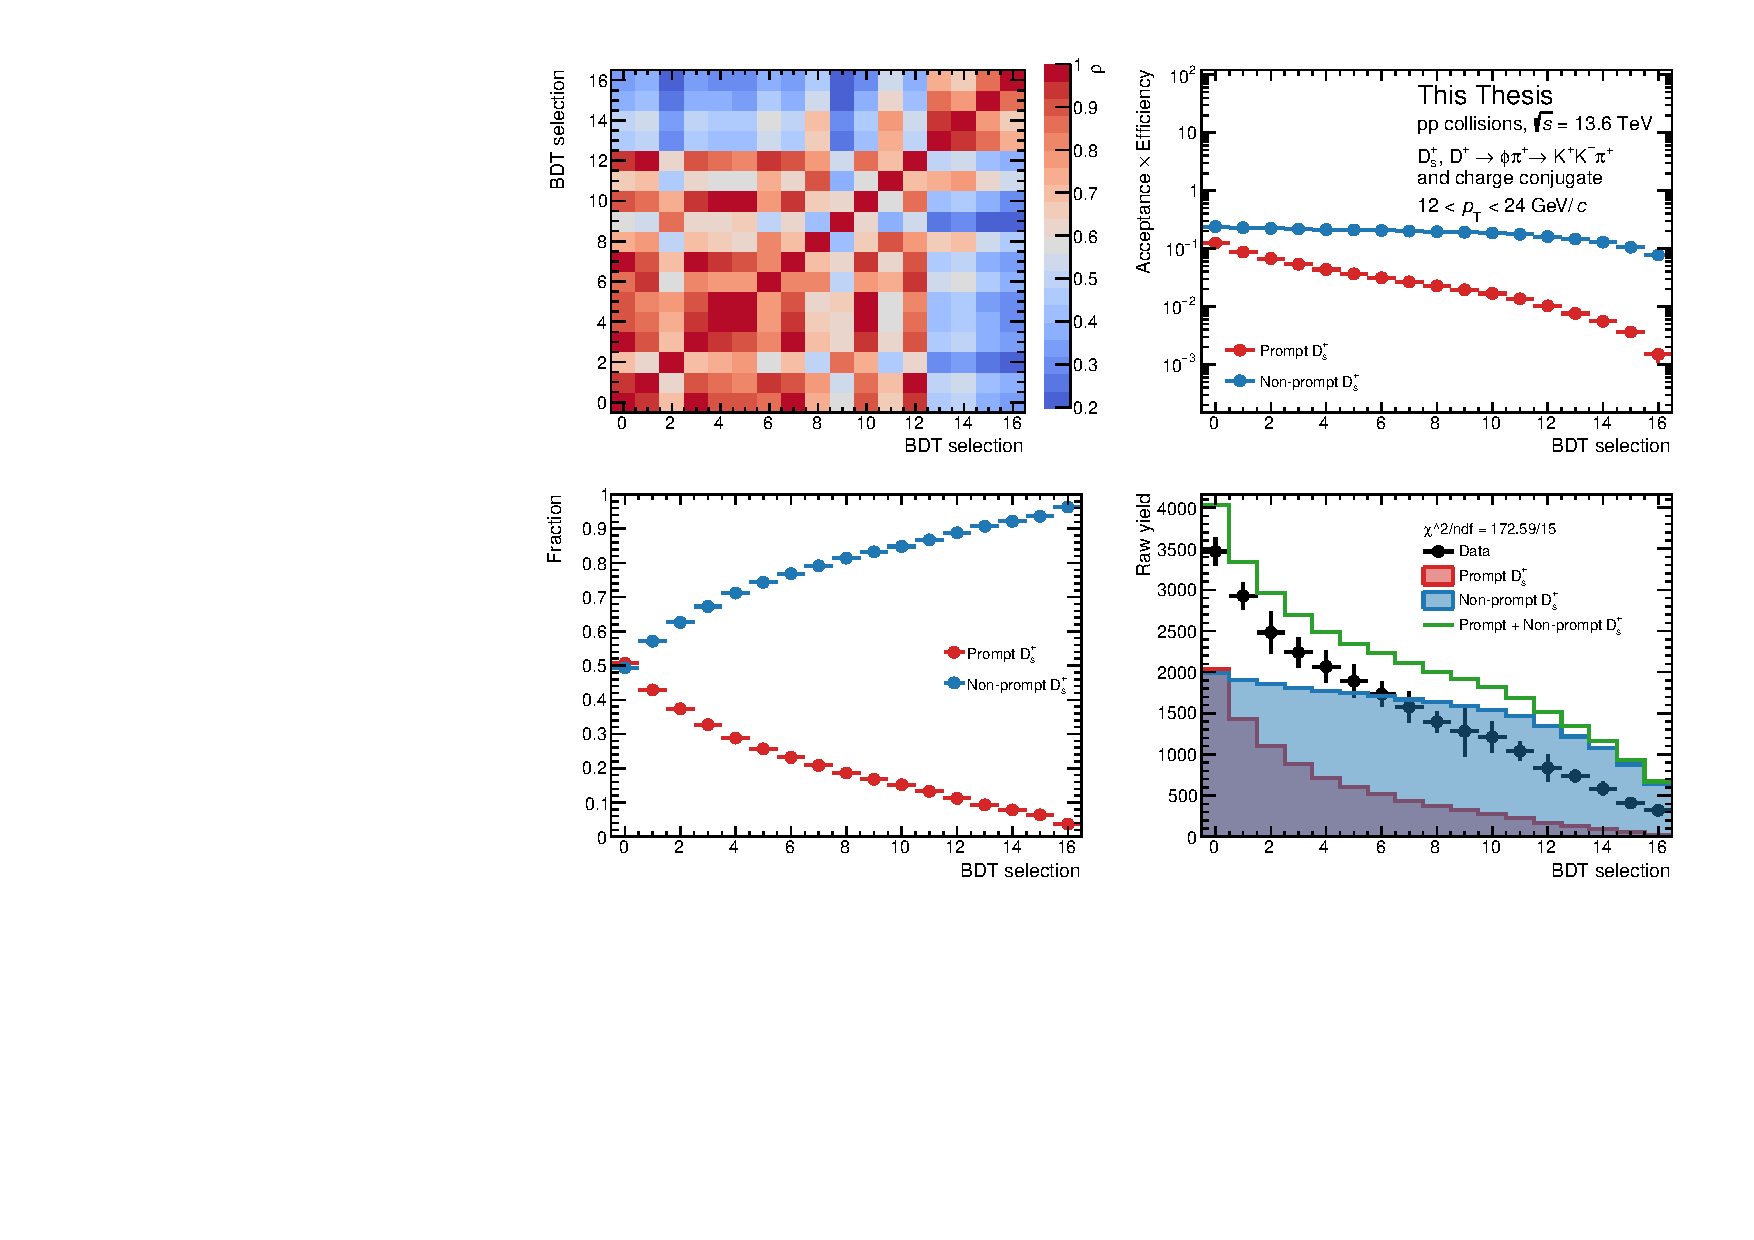
\includegraphics[width=0.7\textwidth]{Figures/Chapter 6/AllPropmtFracs/Ds/DsPromptFrac120_240.pdf}
    \caption{Results for the evaluation of the \fpds correction factor in the $8.0 < \pt < 12.0$~\gevc (top) and $12.0 < \pt < 24.0$~\gevc (bottom) intervals.}
    \end{figure}

\begin{sidewaysfigure}
    \centering
    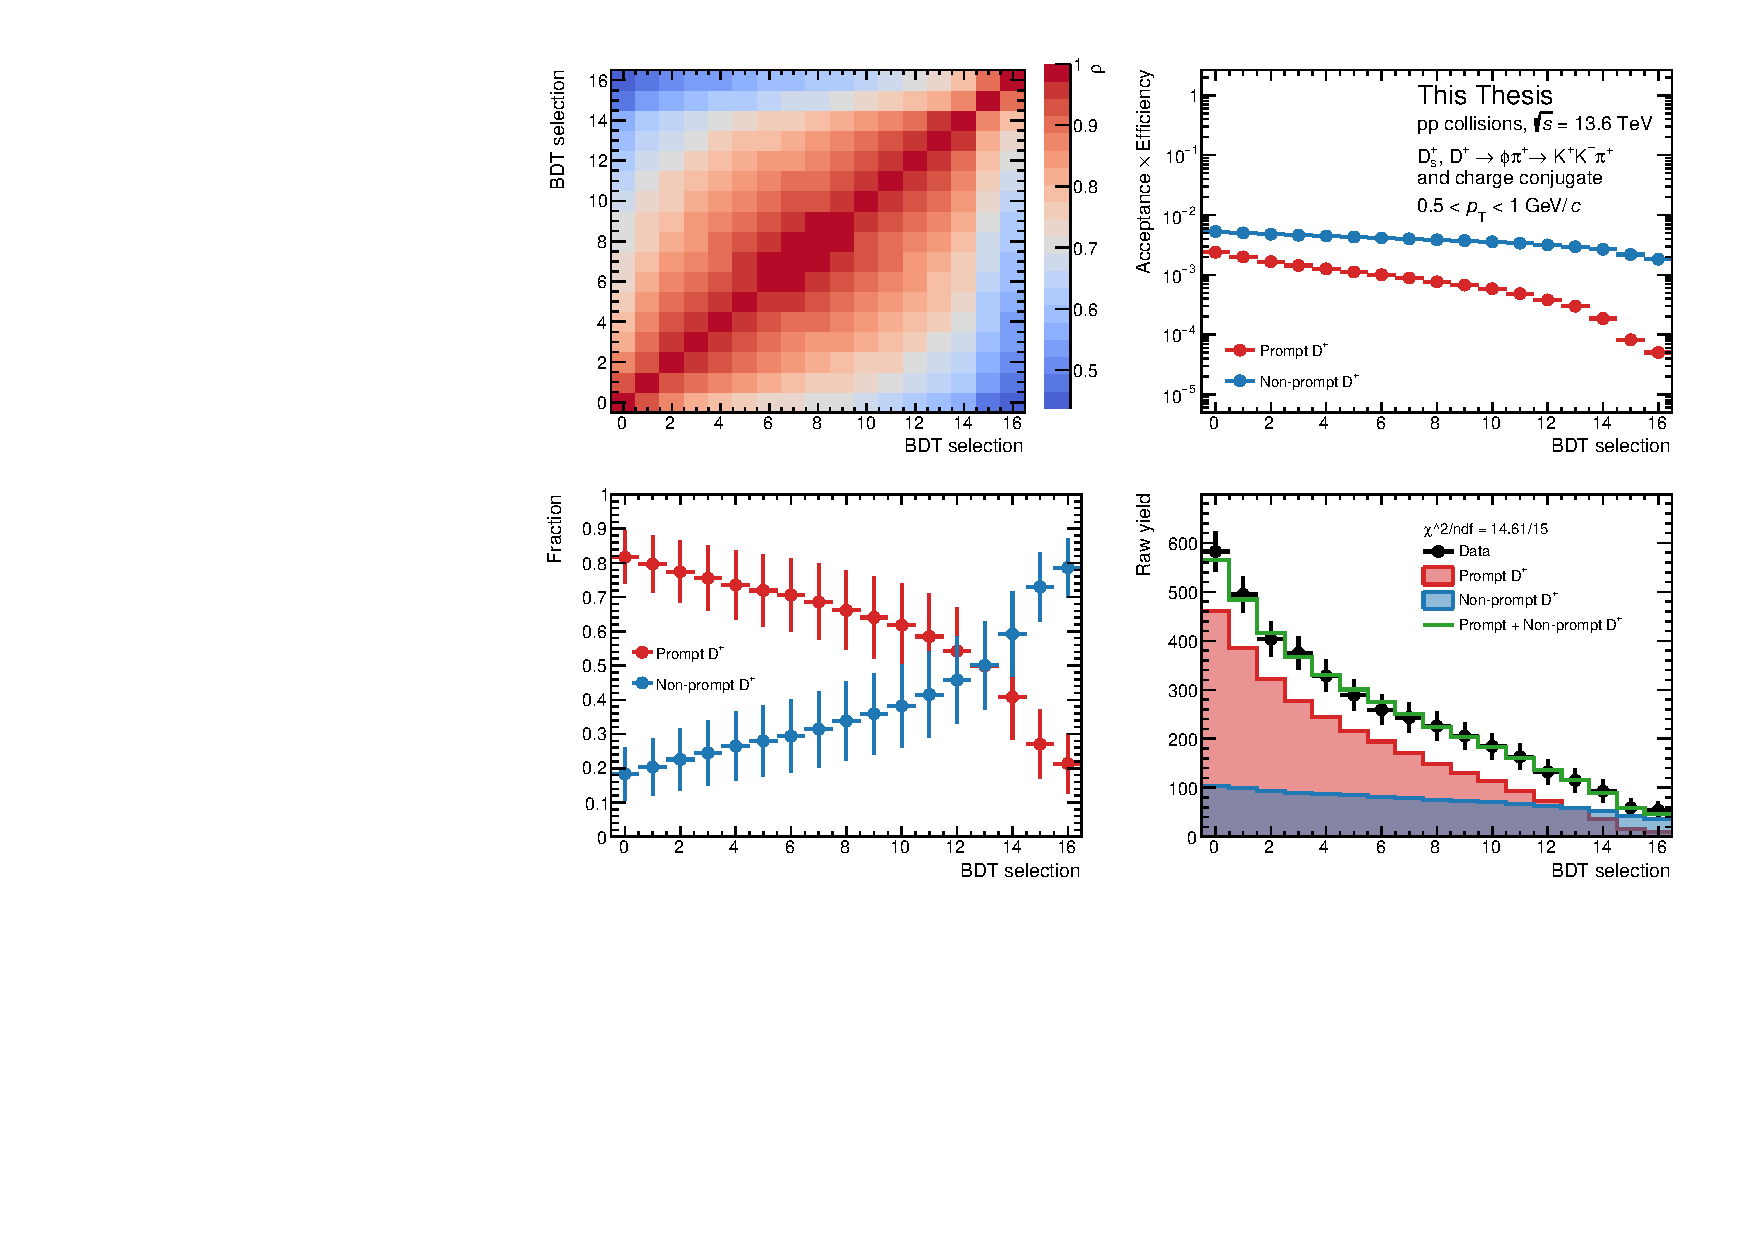
\includegraphics[width=0.48\textwidth]{Figures/Chapter 6/AllPropmtFracs/Dplus/DplusPromptFrac5_10.pdf}
    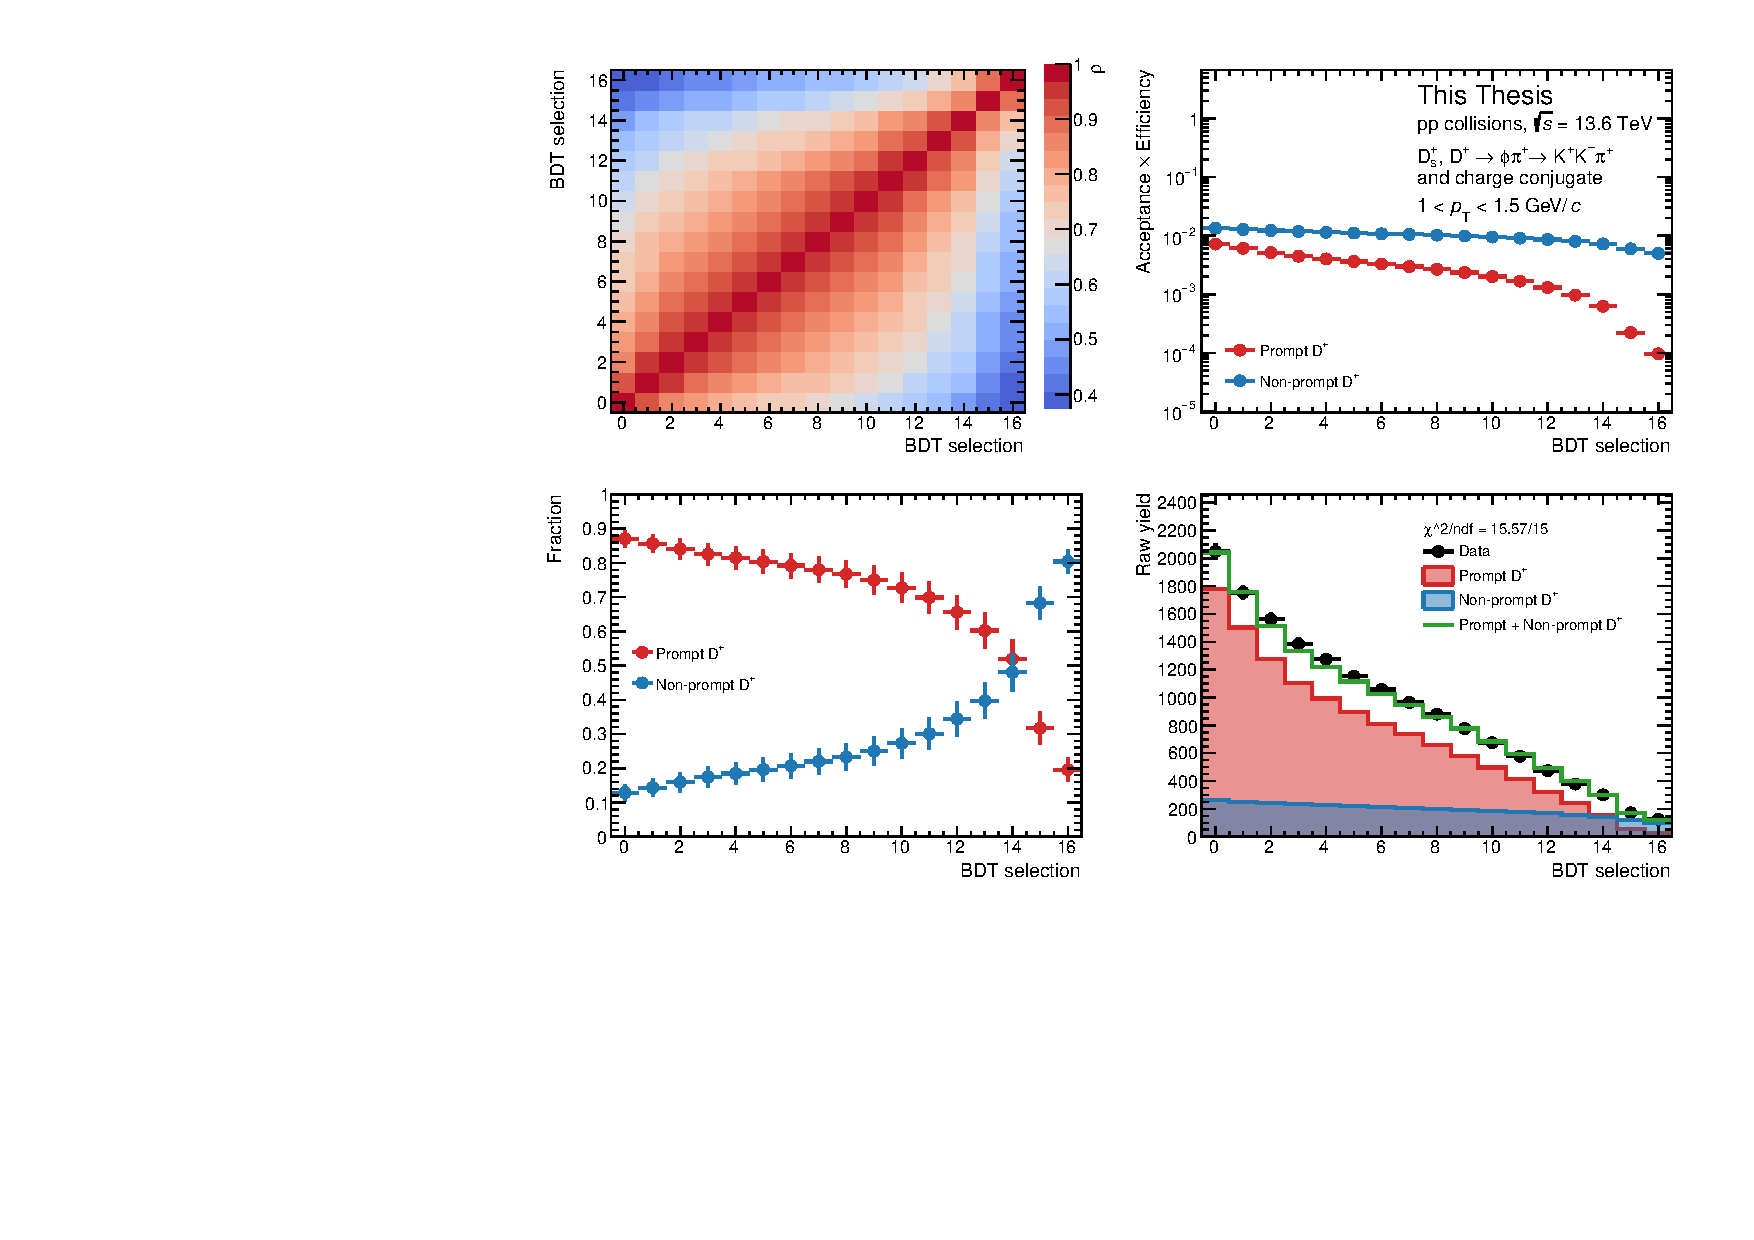
\includegraphics[width=0.48\textwidth]{Figures/Chapter 6/AllPropmtFracs/Dplus/DplusPromptFrac10_15.pdf}
    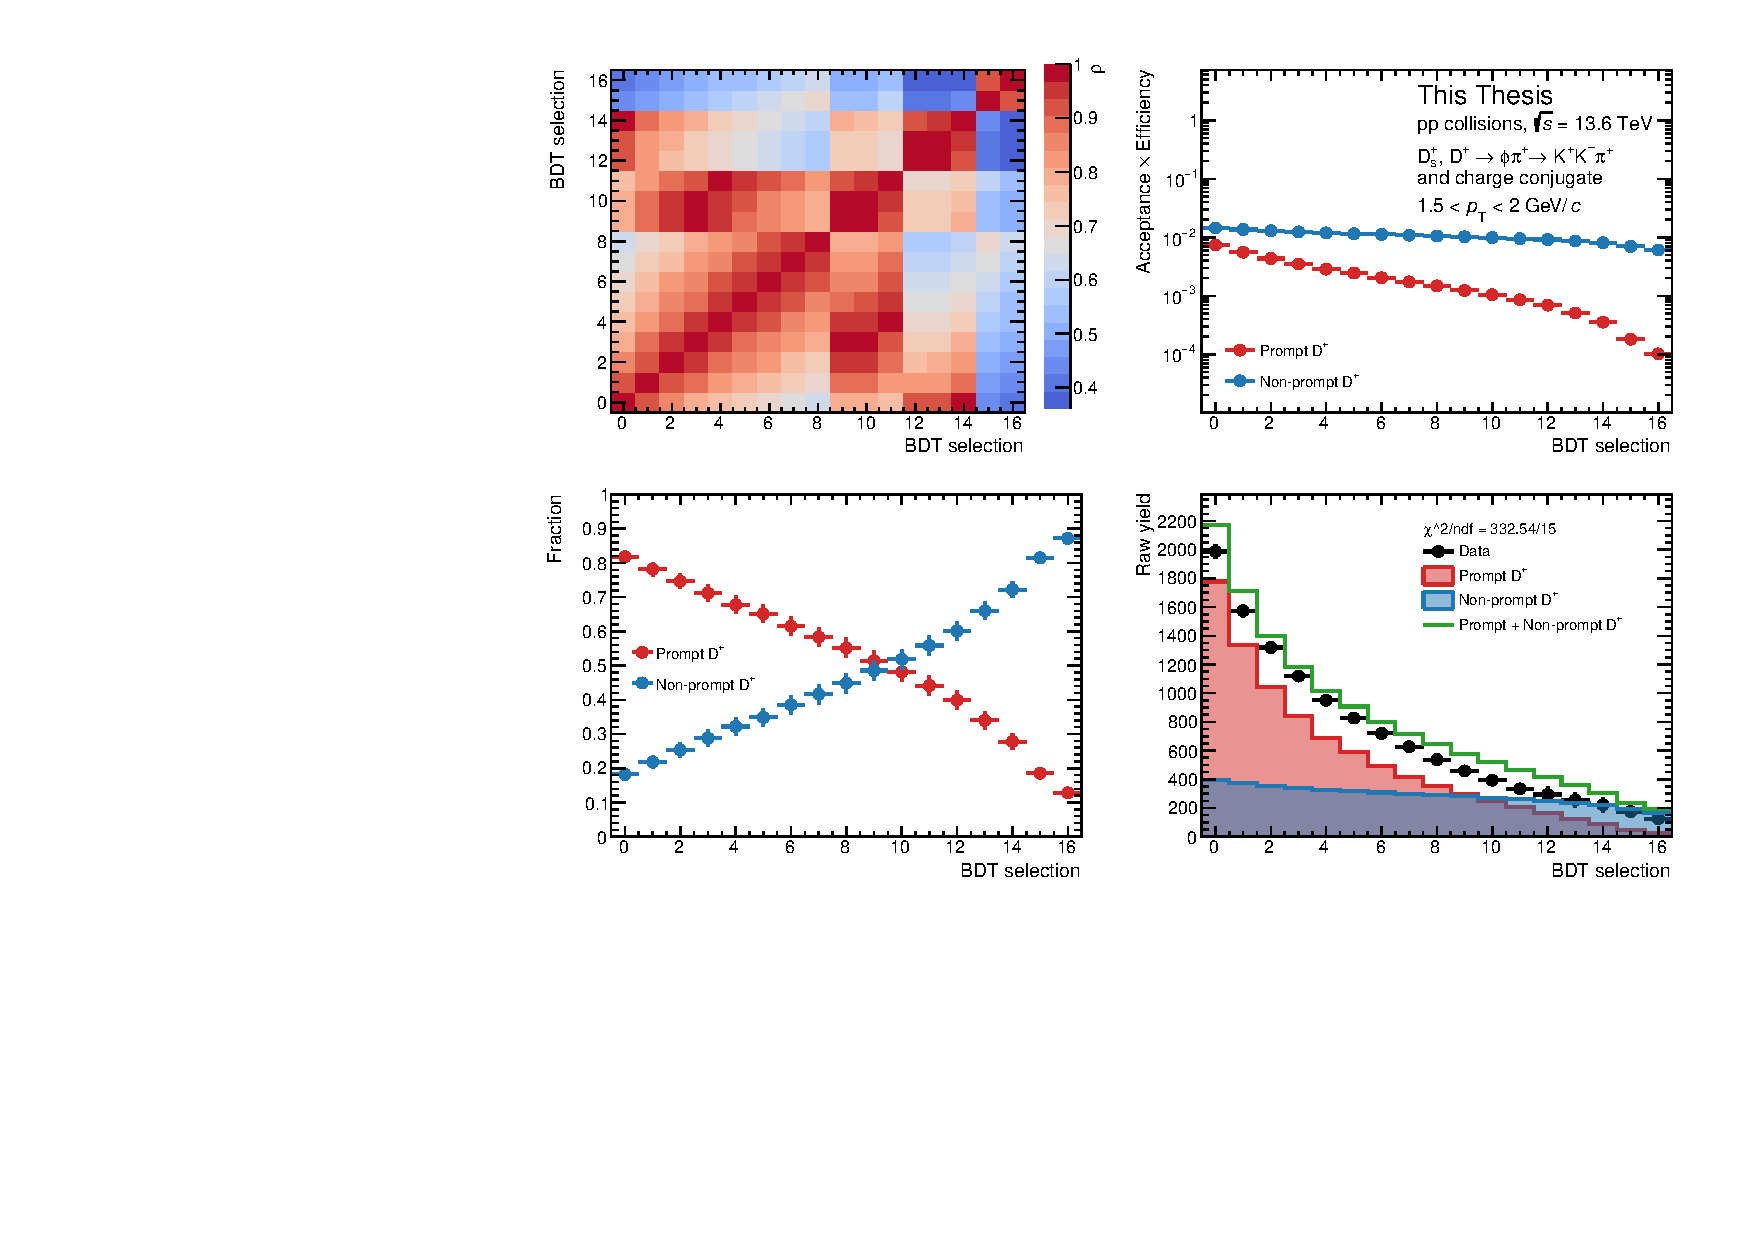
\includegraphics[width=0.48\textwidth]{Figures/Chapter 6/AllPropmtFracs/Dplus/DplusPromptFrac15_20.pdf}
    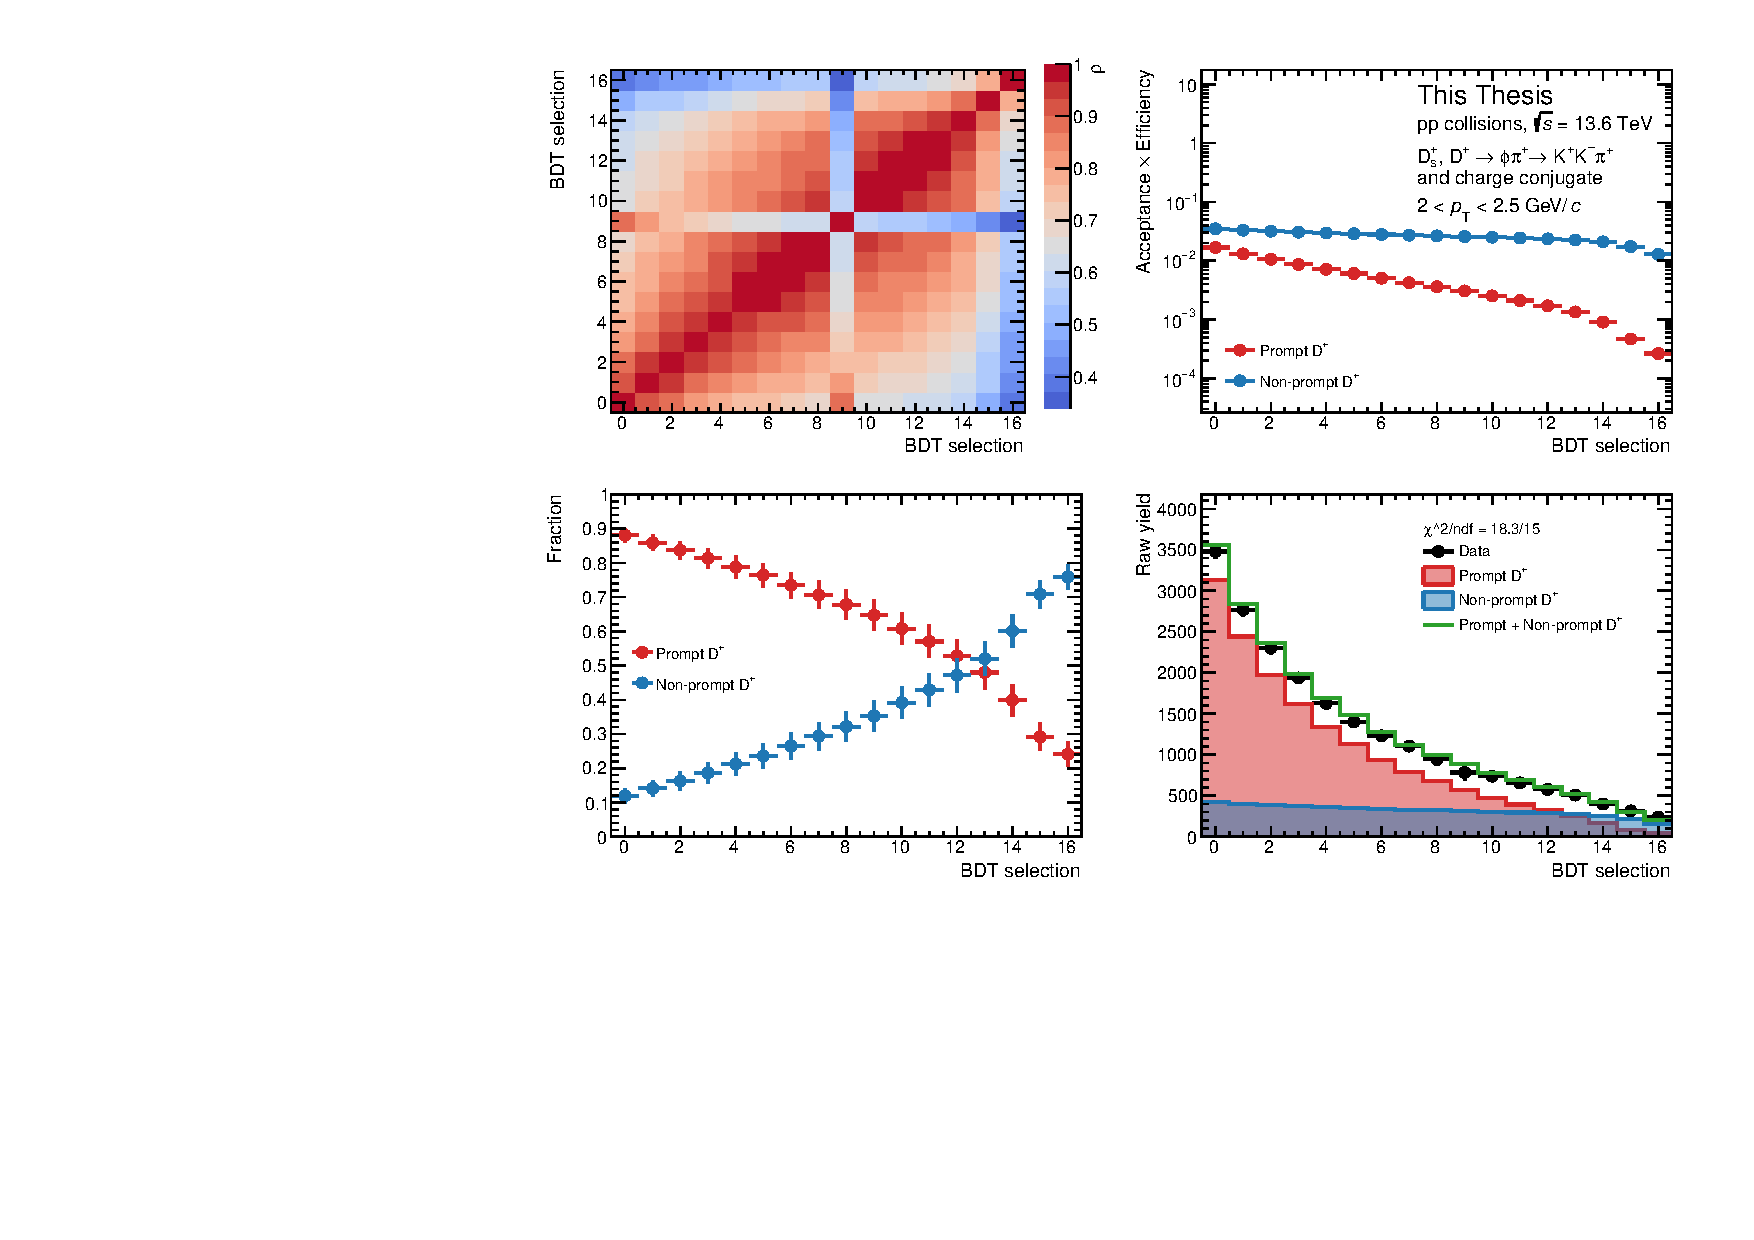
\includegraphics[width=0.48\textwidth]{Figures/Chapter 6/AllPropmtFracs/Dplus/DplusPromptFrac20_25.pdf}
    \caption{Results for the evaluation of the \fpdpl correction factor in the $0.5 < \pt < 1.0$~\gevc (top left), $1.0 < \pt < 1.5$~\gevc (top right), $1.5 < \pt < 2.0$~\gevc (bottom left) and $2.0 < \pt < 2.5$~\gevc (bottom right) intervals.}
\end{sidewaysfigure}

\begin{sidewaysfigure}
    \centering
    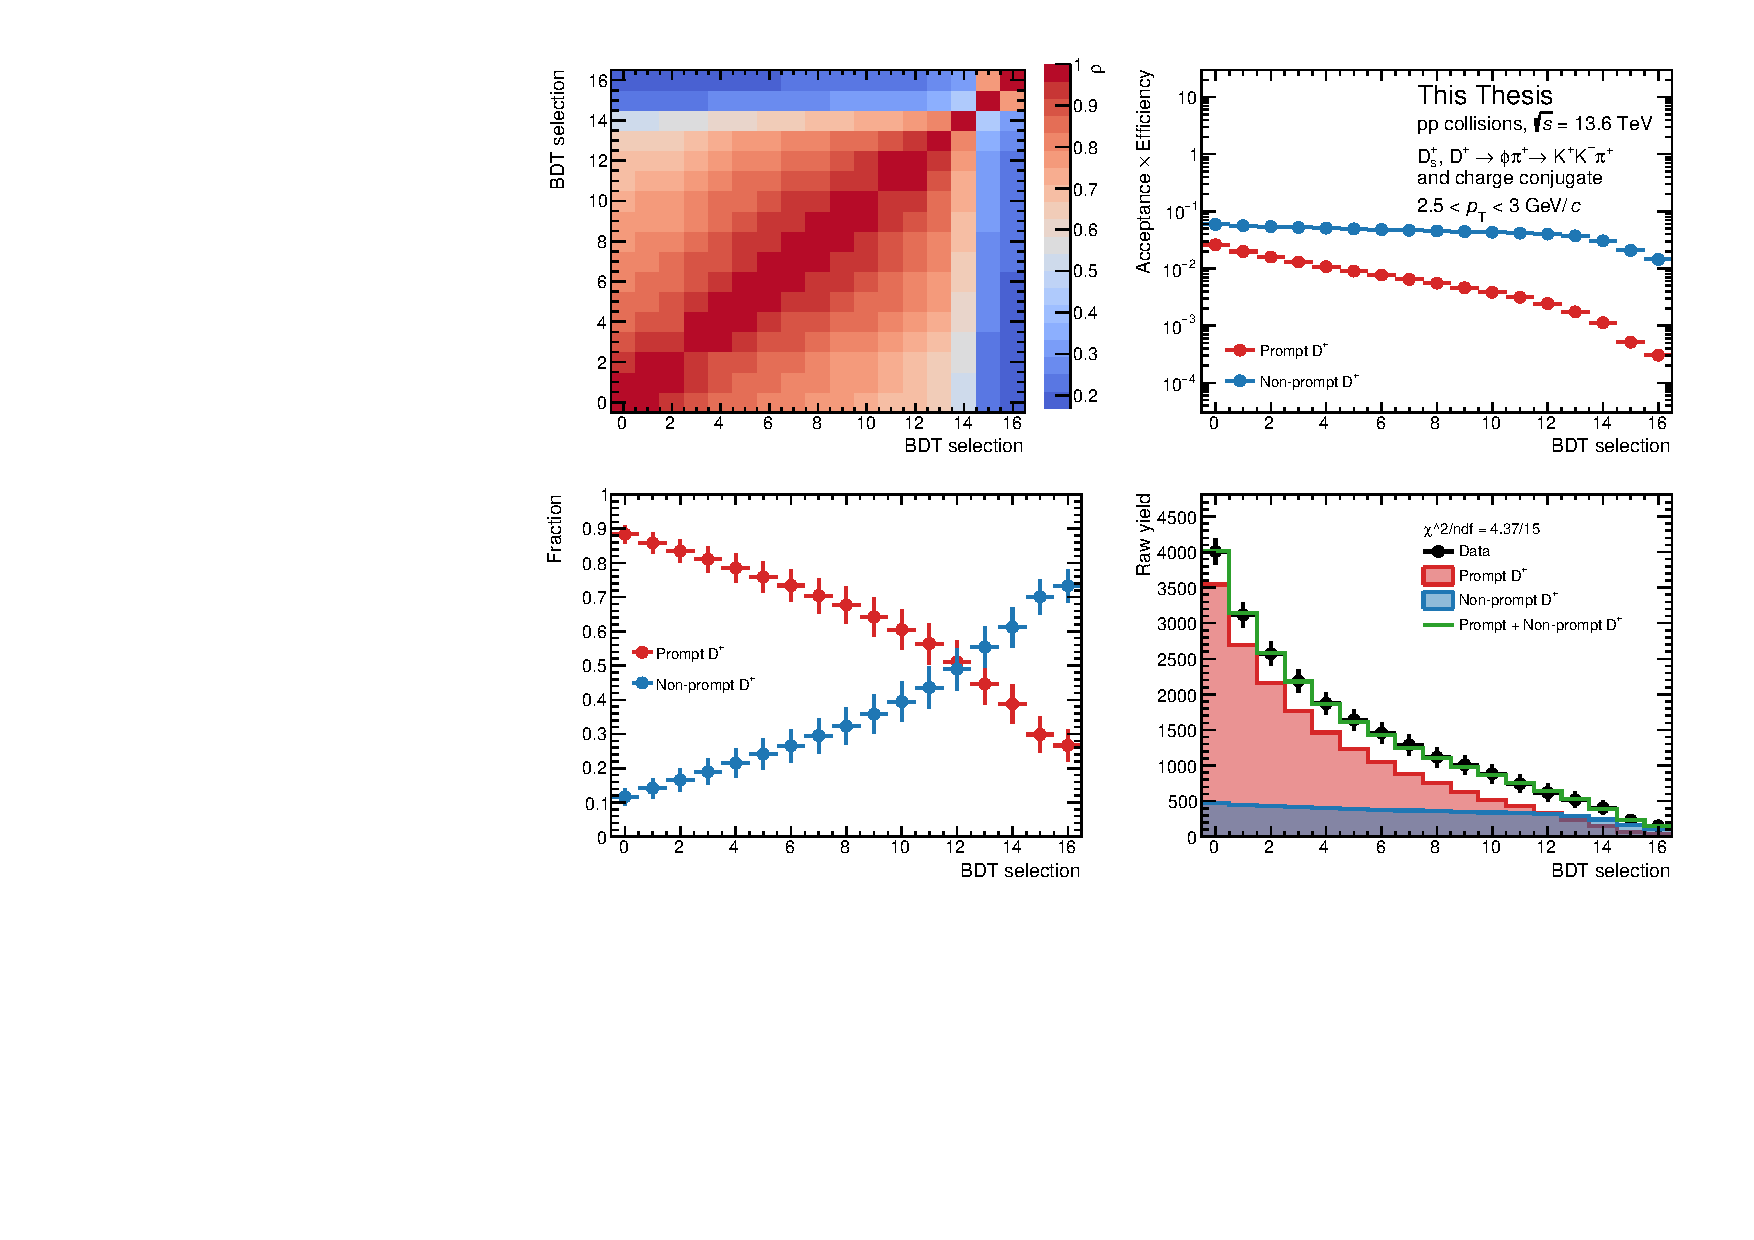
\includegraphics[width=0.48\textwidth]{Figures/Chapter 6/AllPropmtFracs/Dplus/DplusPromptFrac25_30.pdf}
    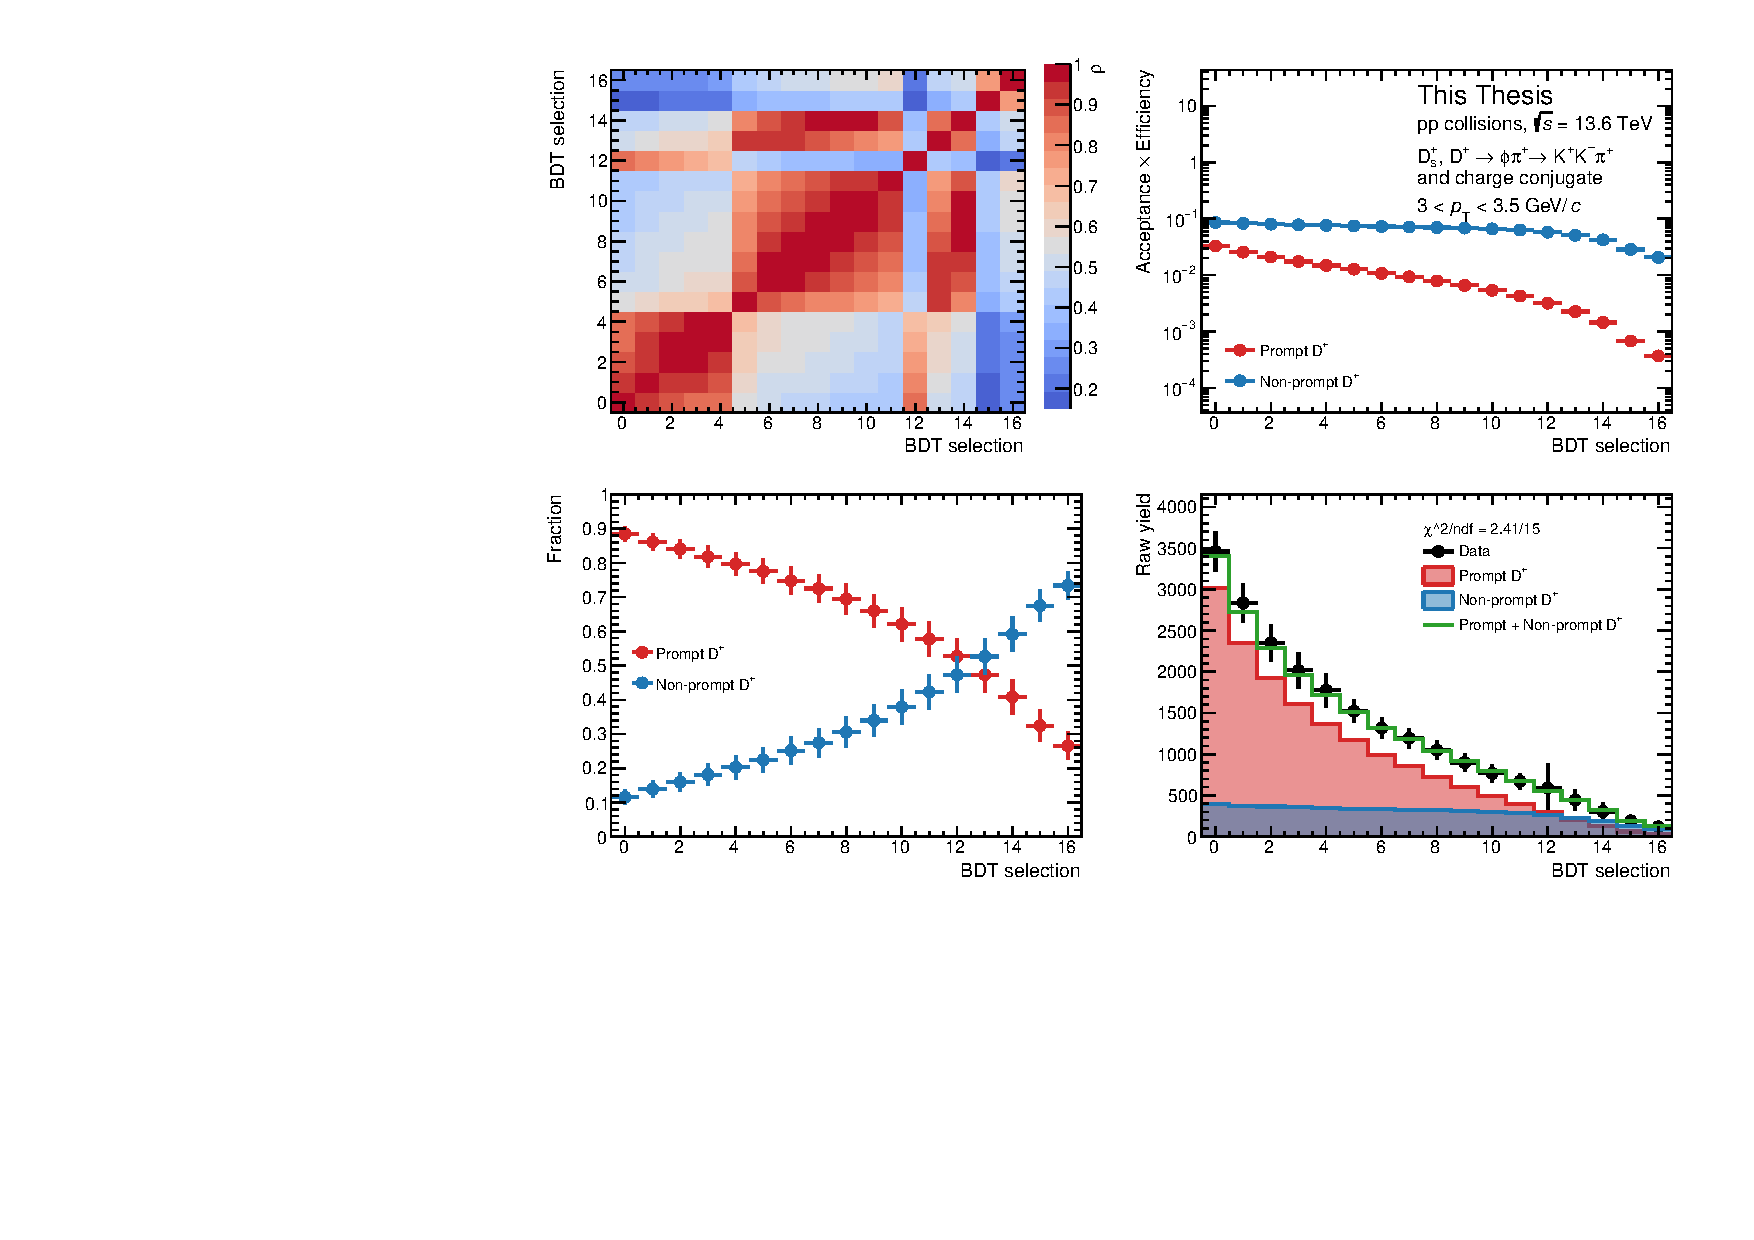
\includegraphics[width=0.48\textwidth]{Figures/Chapter 6/AllPropmtFracs/Dplus/DplusPromptFrac30_35.pdf}
    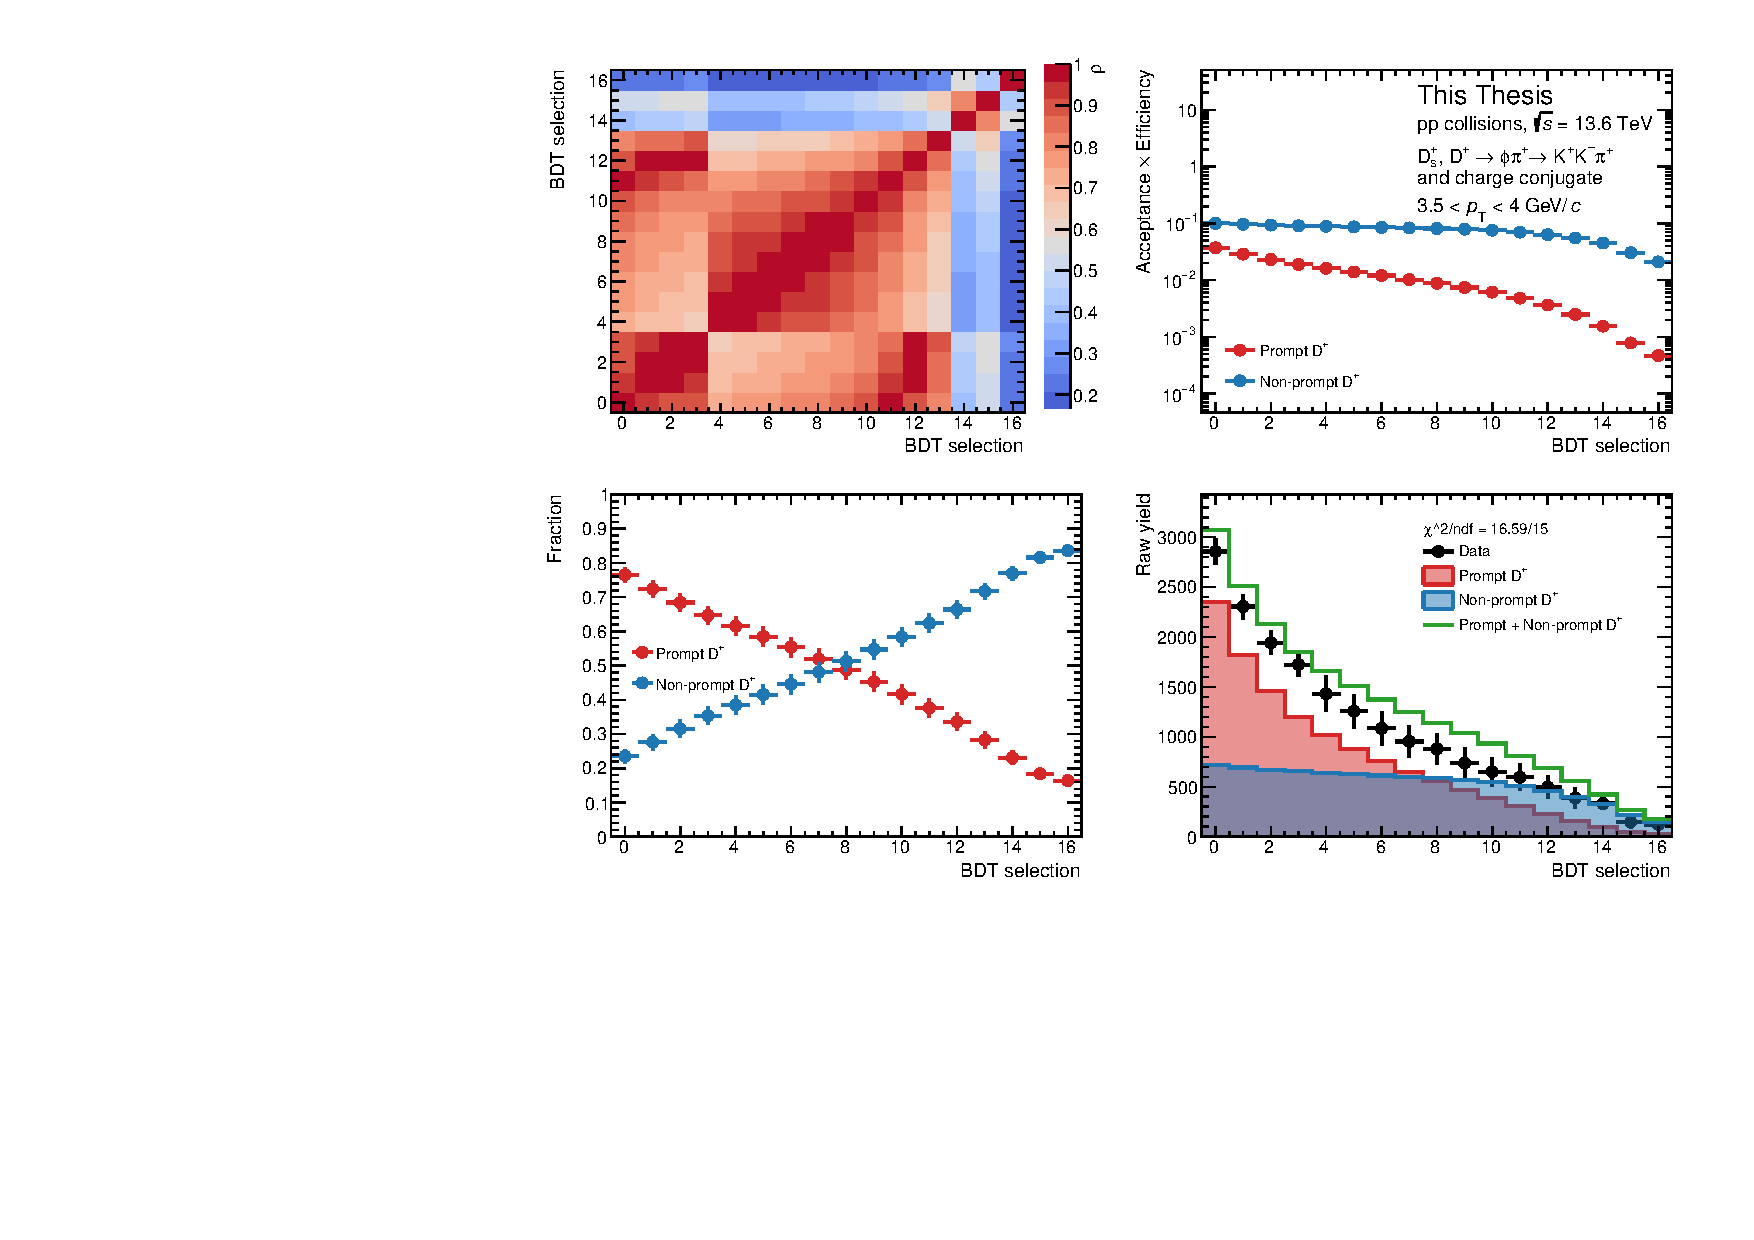
\includegraphics[width=0.48\textwidth]{Figures/Chapter 6/AllPropmtFracs/Dplus/DplusPromptFrac35_40.pdf}
    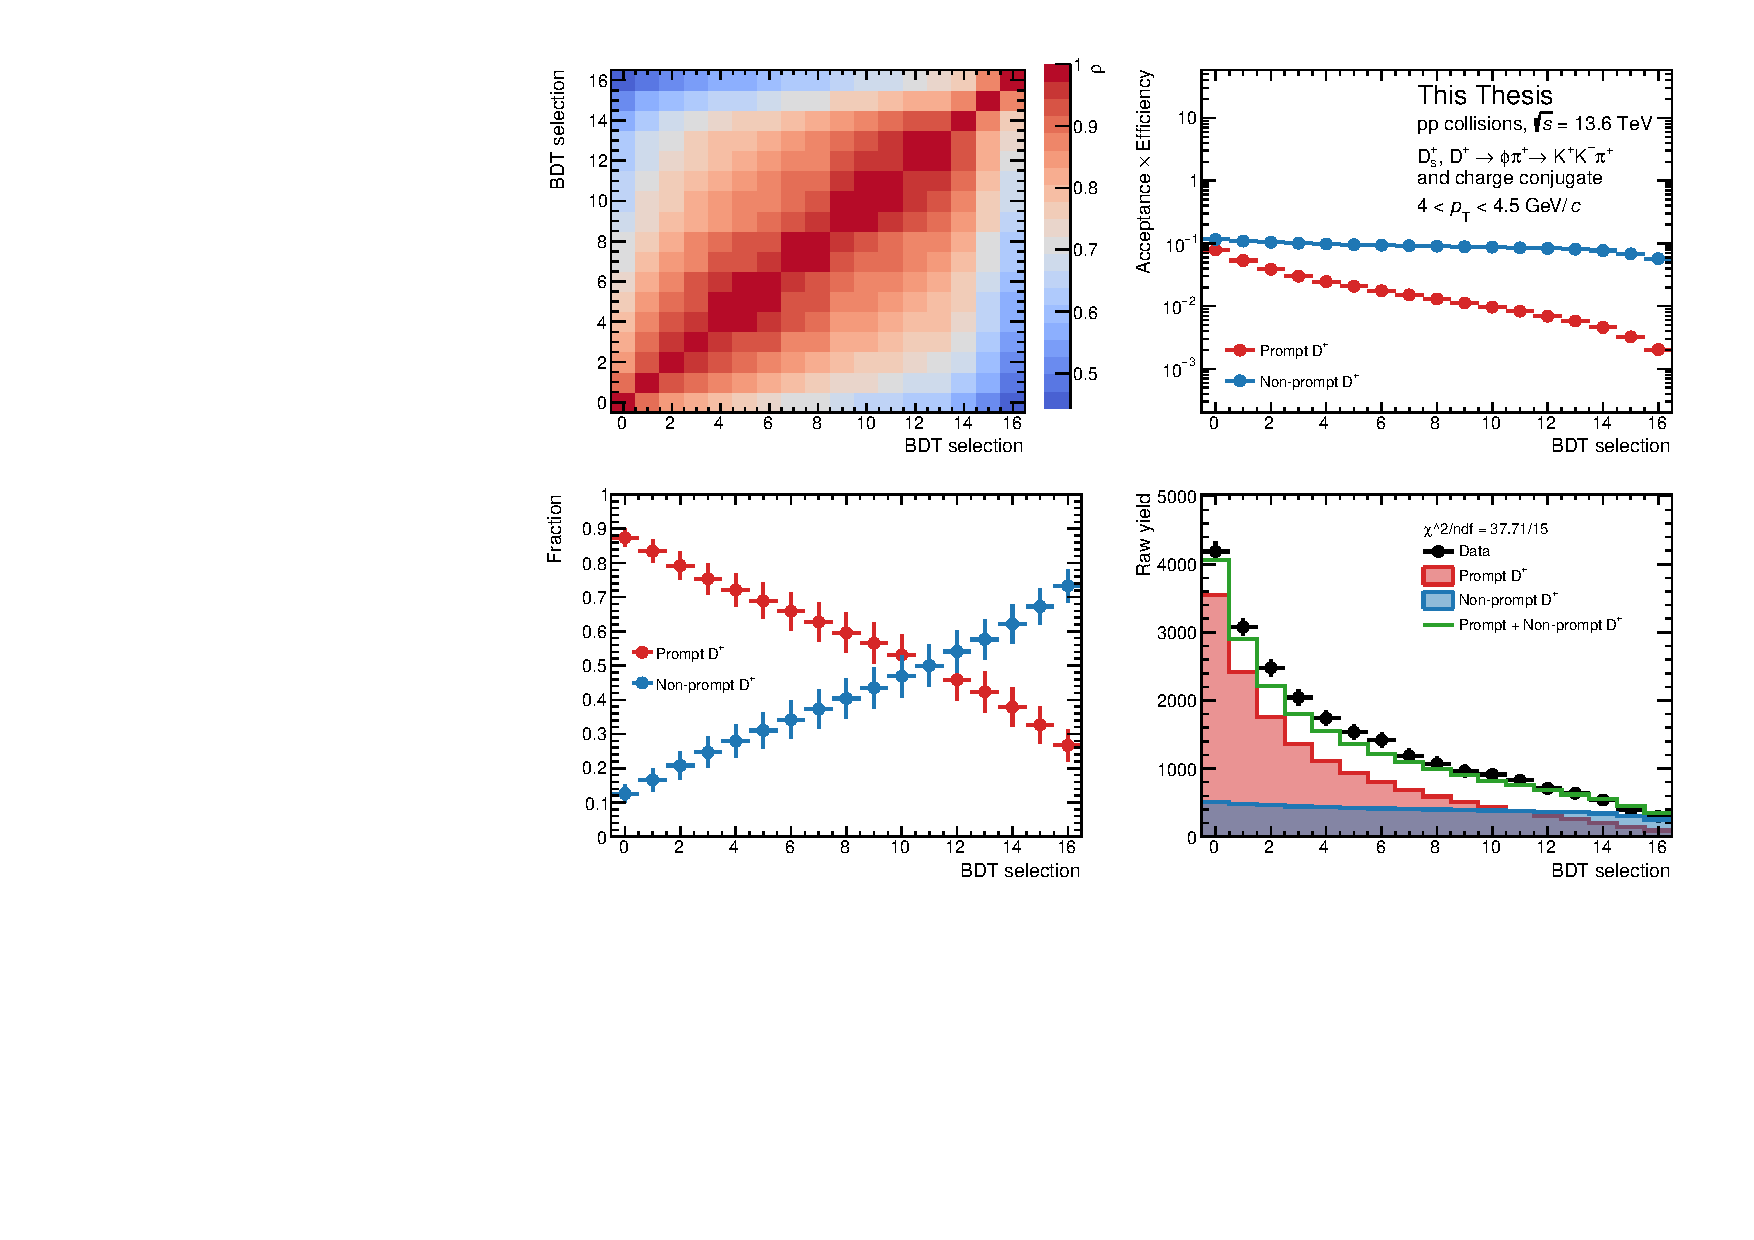
\includegraphics[width=0.48\textwidth]{Figures/Chapter 6/AllPropmtFracs/Dplus/DplusPromptFrac40_45.pdf}
    \caption{Results for the evaluation of the \fpdpl correction factor in the $2.5 < \pt < 3.0$~\gevc (top left), $3.0 < \pt < 3.5$~\gevc (top right), $3.5 < \pt < 4.0$~\gevc (bottom left) and $4.0 < \pt < 4.5$~\gevc (bottom right) intervals.}
\end{sidewaysfigure}

\begin{sidewaysfigure}
    \centering
    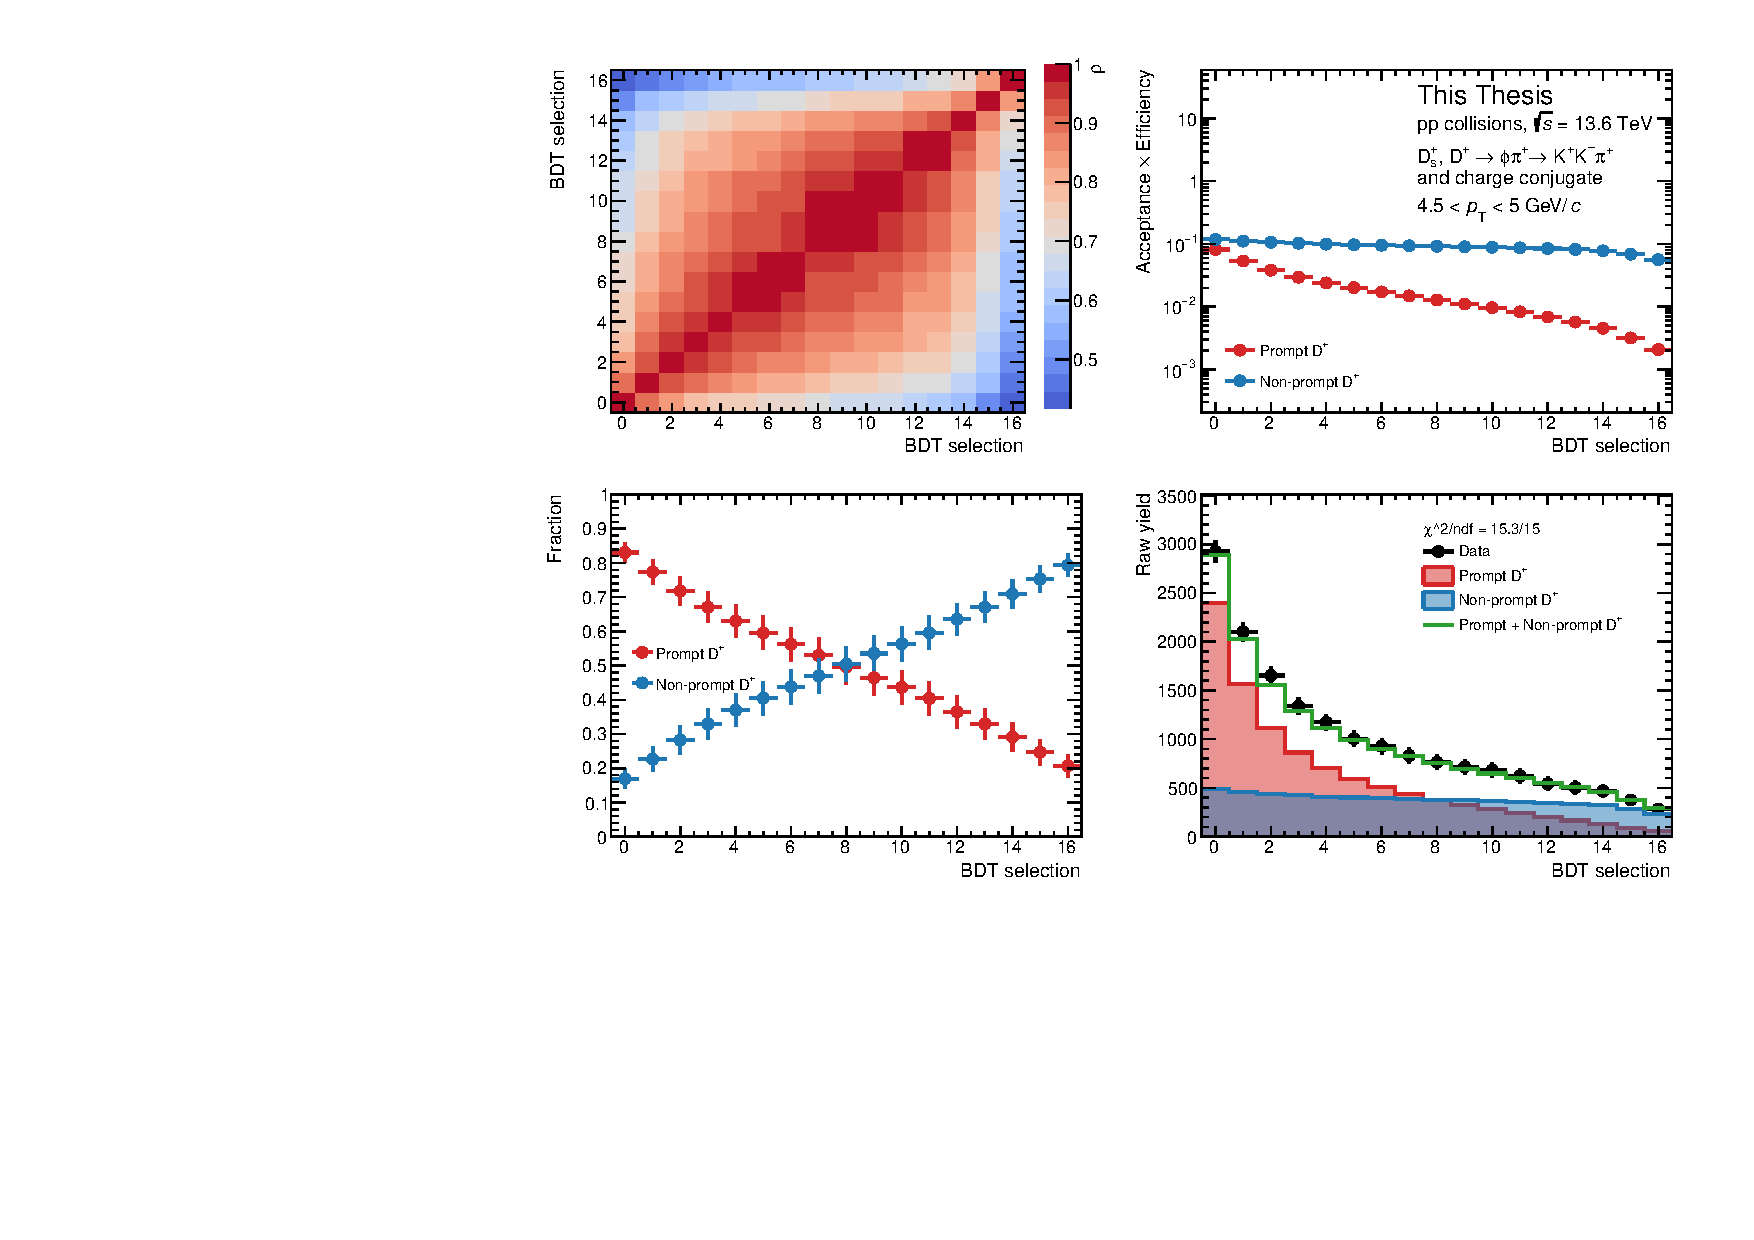
\includegraphics[width=0.48\textwidth]{Figures/Chapter 6/AllPropmtFracs/Dplus/DplusPromptFrac45_50.pdf}
    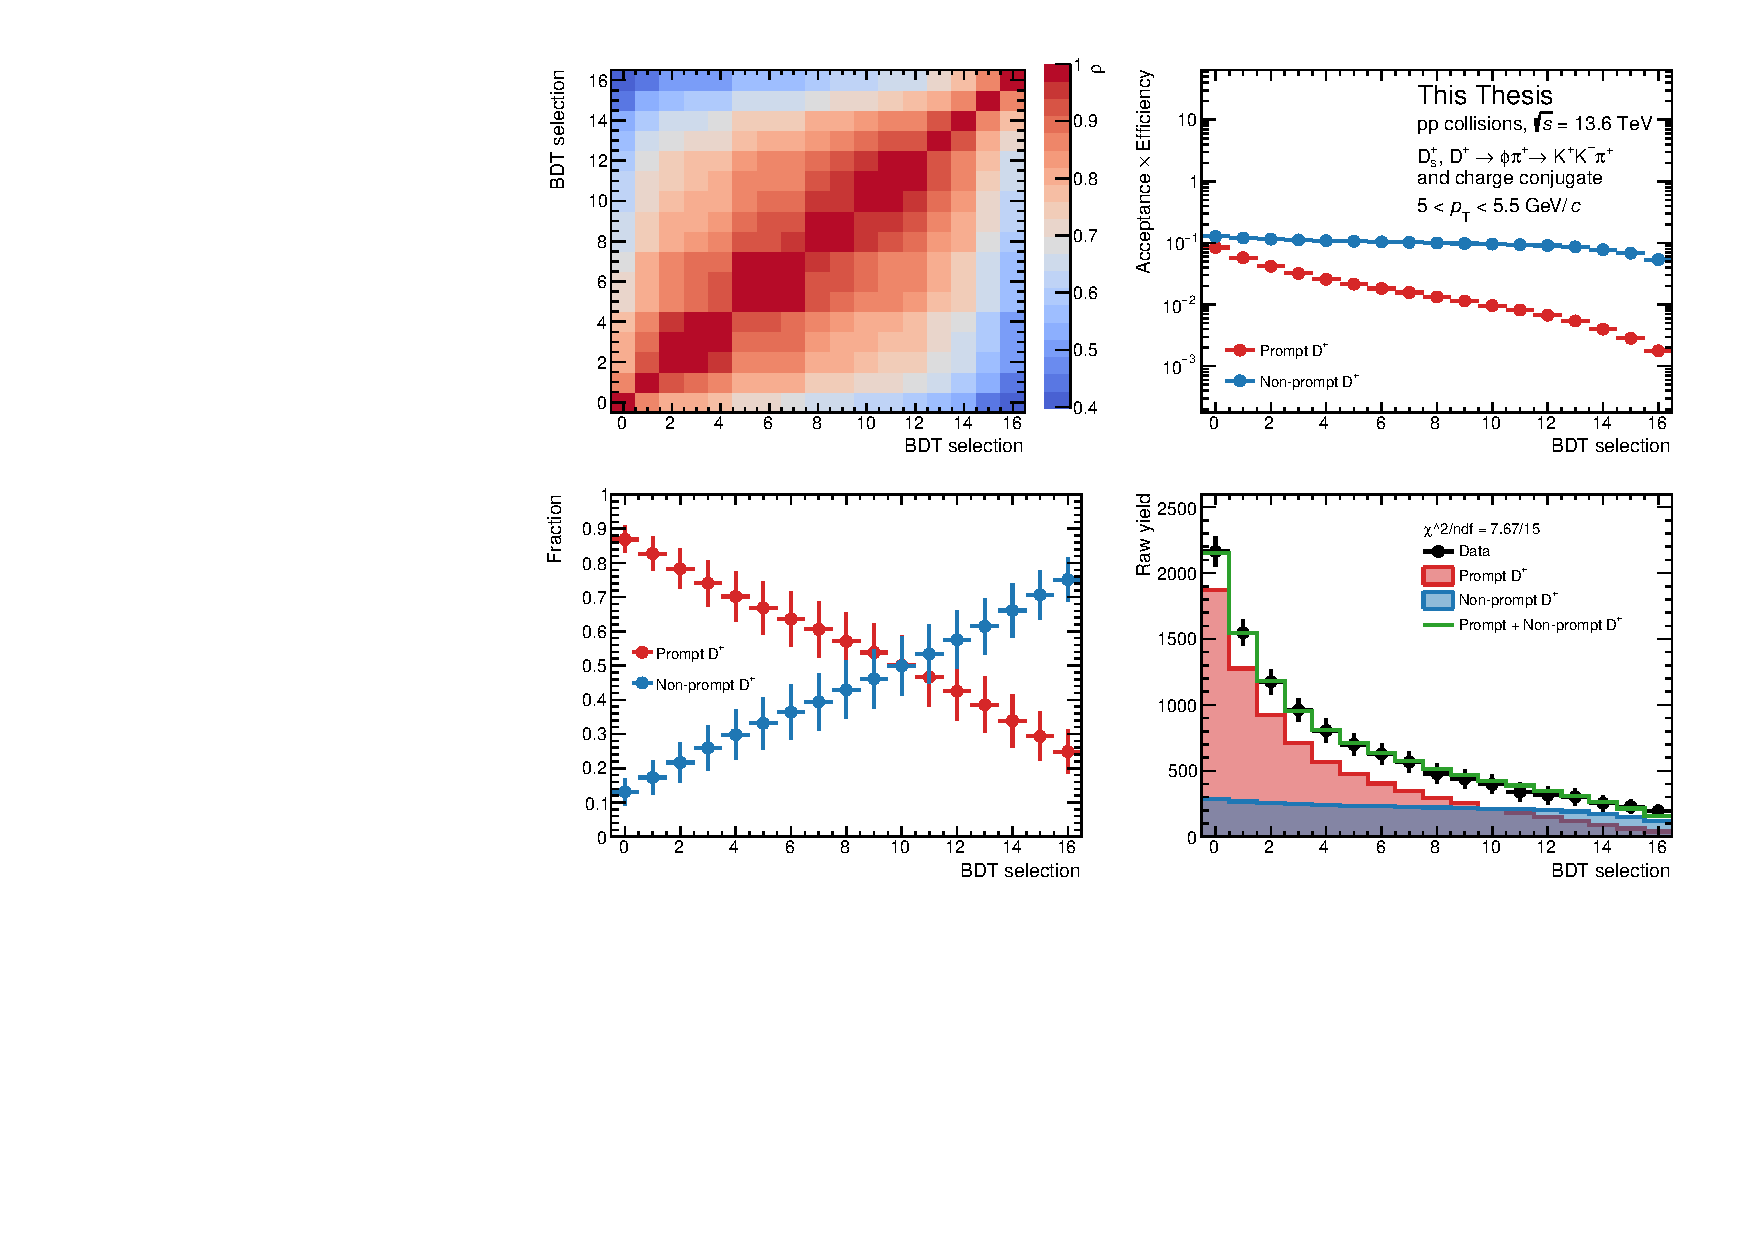
\includegraphics[width=0.48\textwidth]{Figures/Chapter 6/AllPropmtFracs/Dplus/DplusPromptFrac50_55.pdf}
    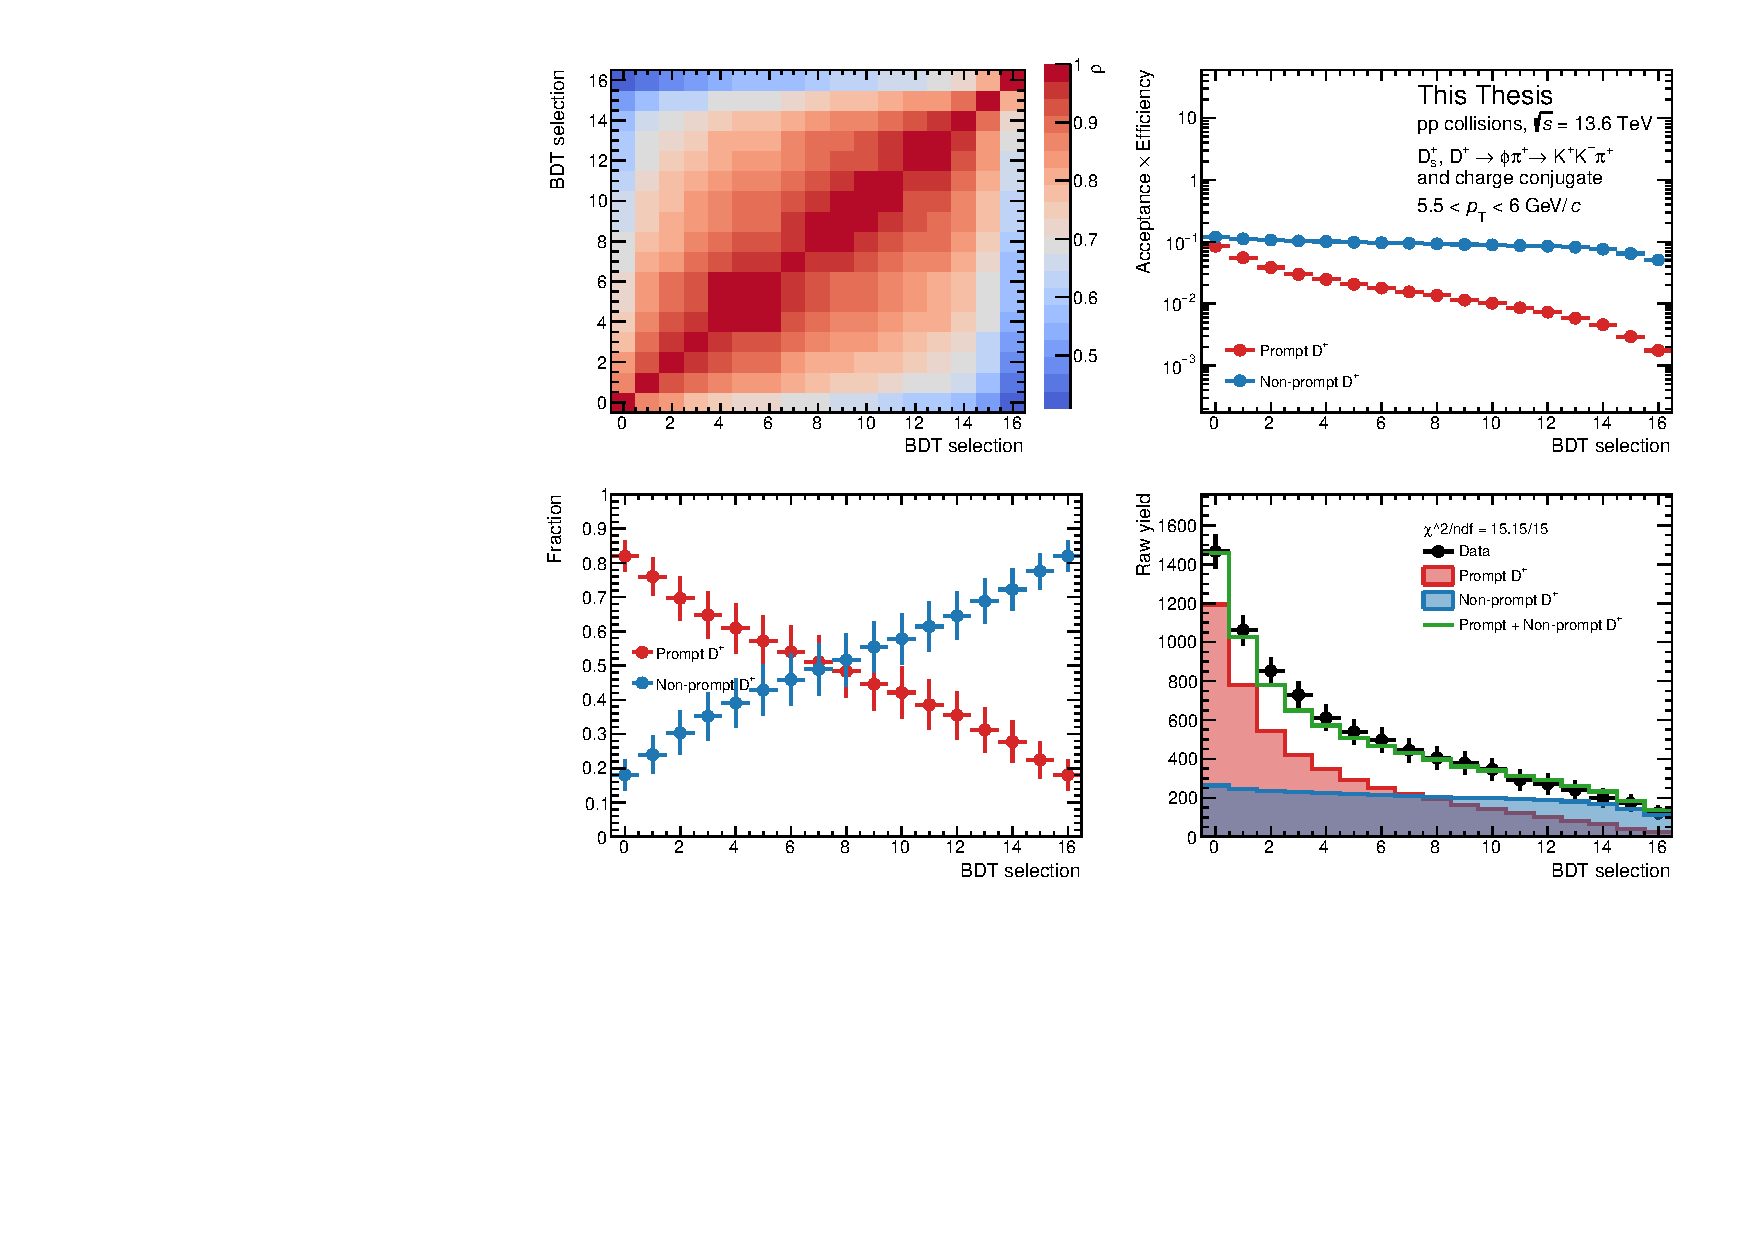
\includegraphics[width=0.48\textwidth]{Figures/Chapter 6/AllPropmtFracs/Dplus/DplusPromptFrac55_60.pdf}
    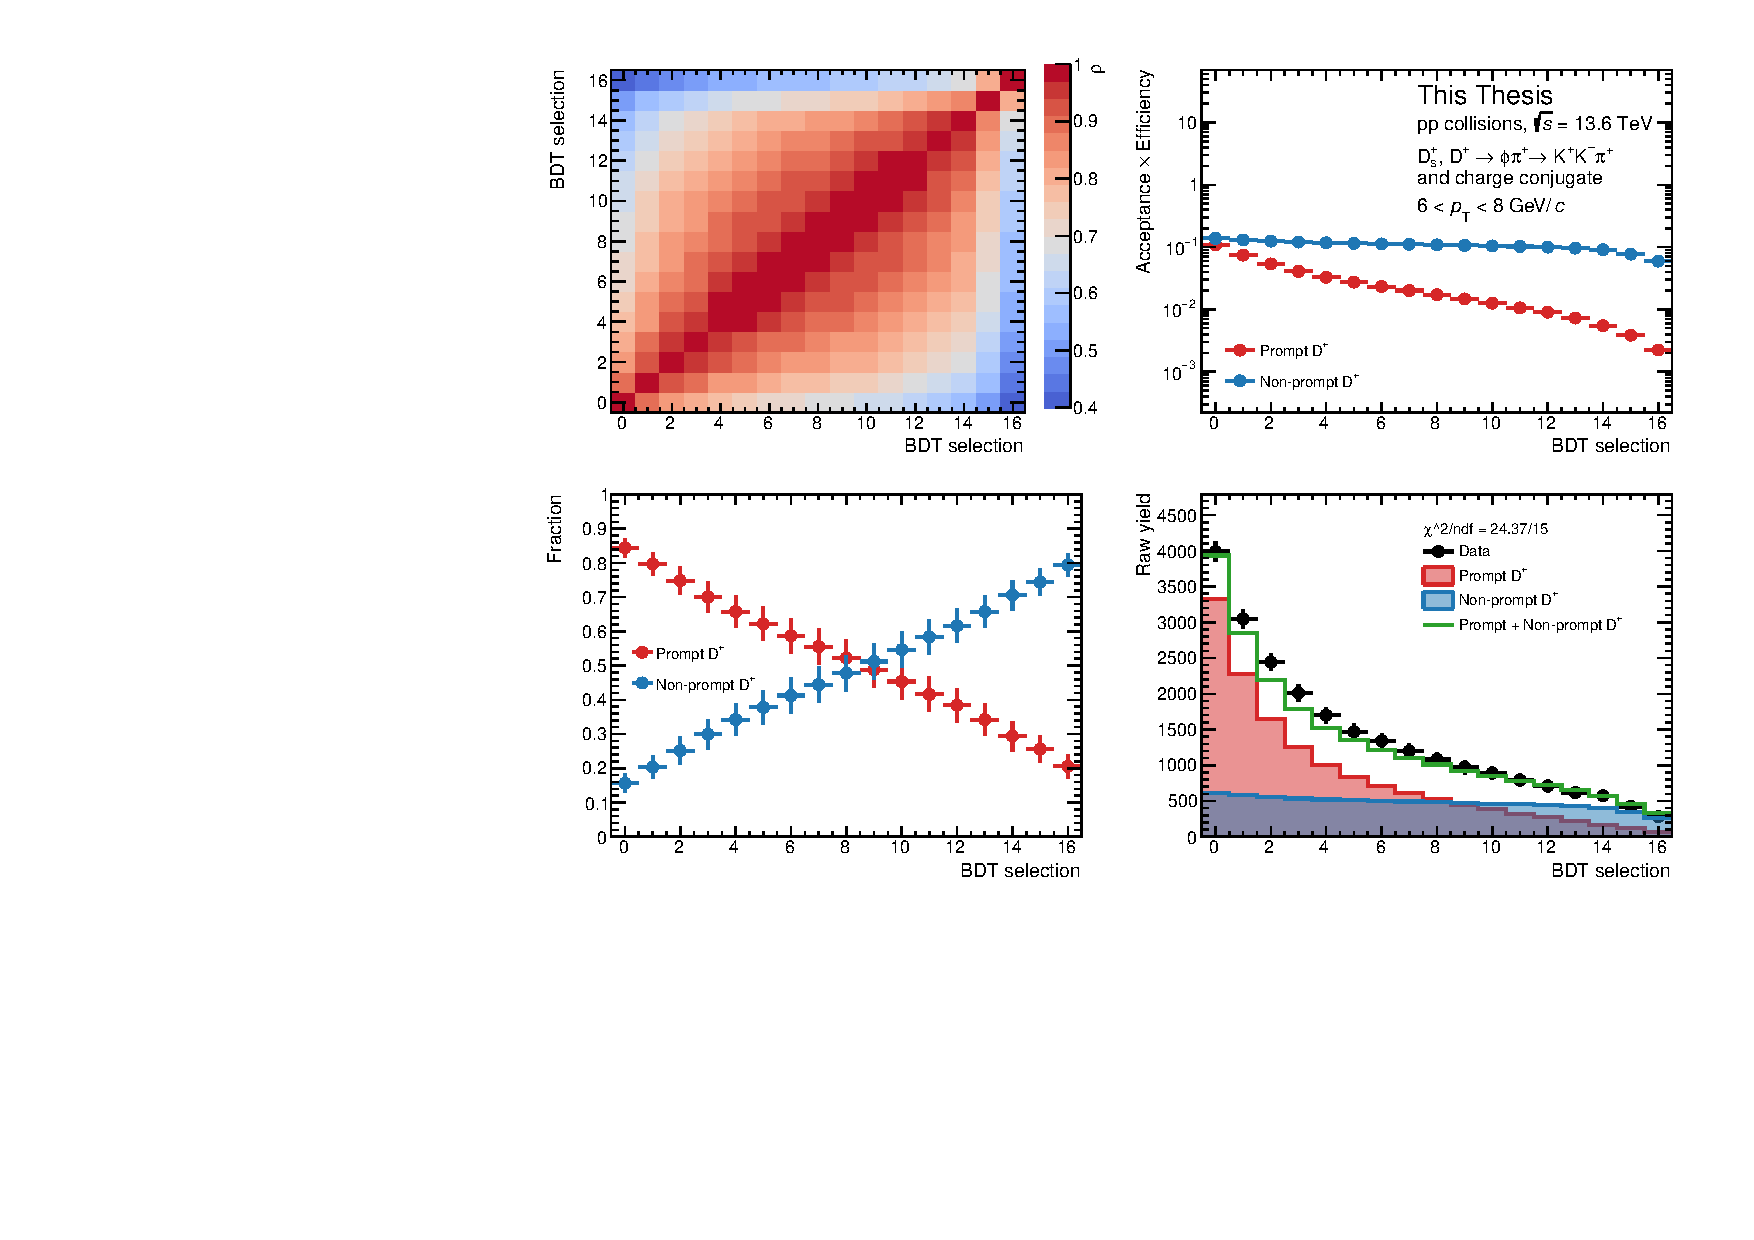
\includegraphics[width=0.48\textwidth]{Figures/Chapter 6/AllPropmtFracs/Dplus/DplusPromptFrac60_80.pdf}
    \caption{Results for the evaluation of the \fpdpl correction factor in the $4.5 < \pt < 5.0$~\gevc (top left), $5.0 < \pt < 5.5$~\gevc (top right), $5.5 < \pt < 6.0$~\gevc (bottom left) and $6.0 < \pt < 8.0$~\gevc (bottom right) intervals.}
\end{sidewaysfigure}

\begin{figure}
    \centering
    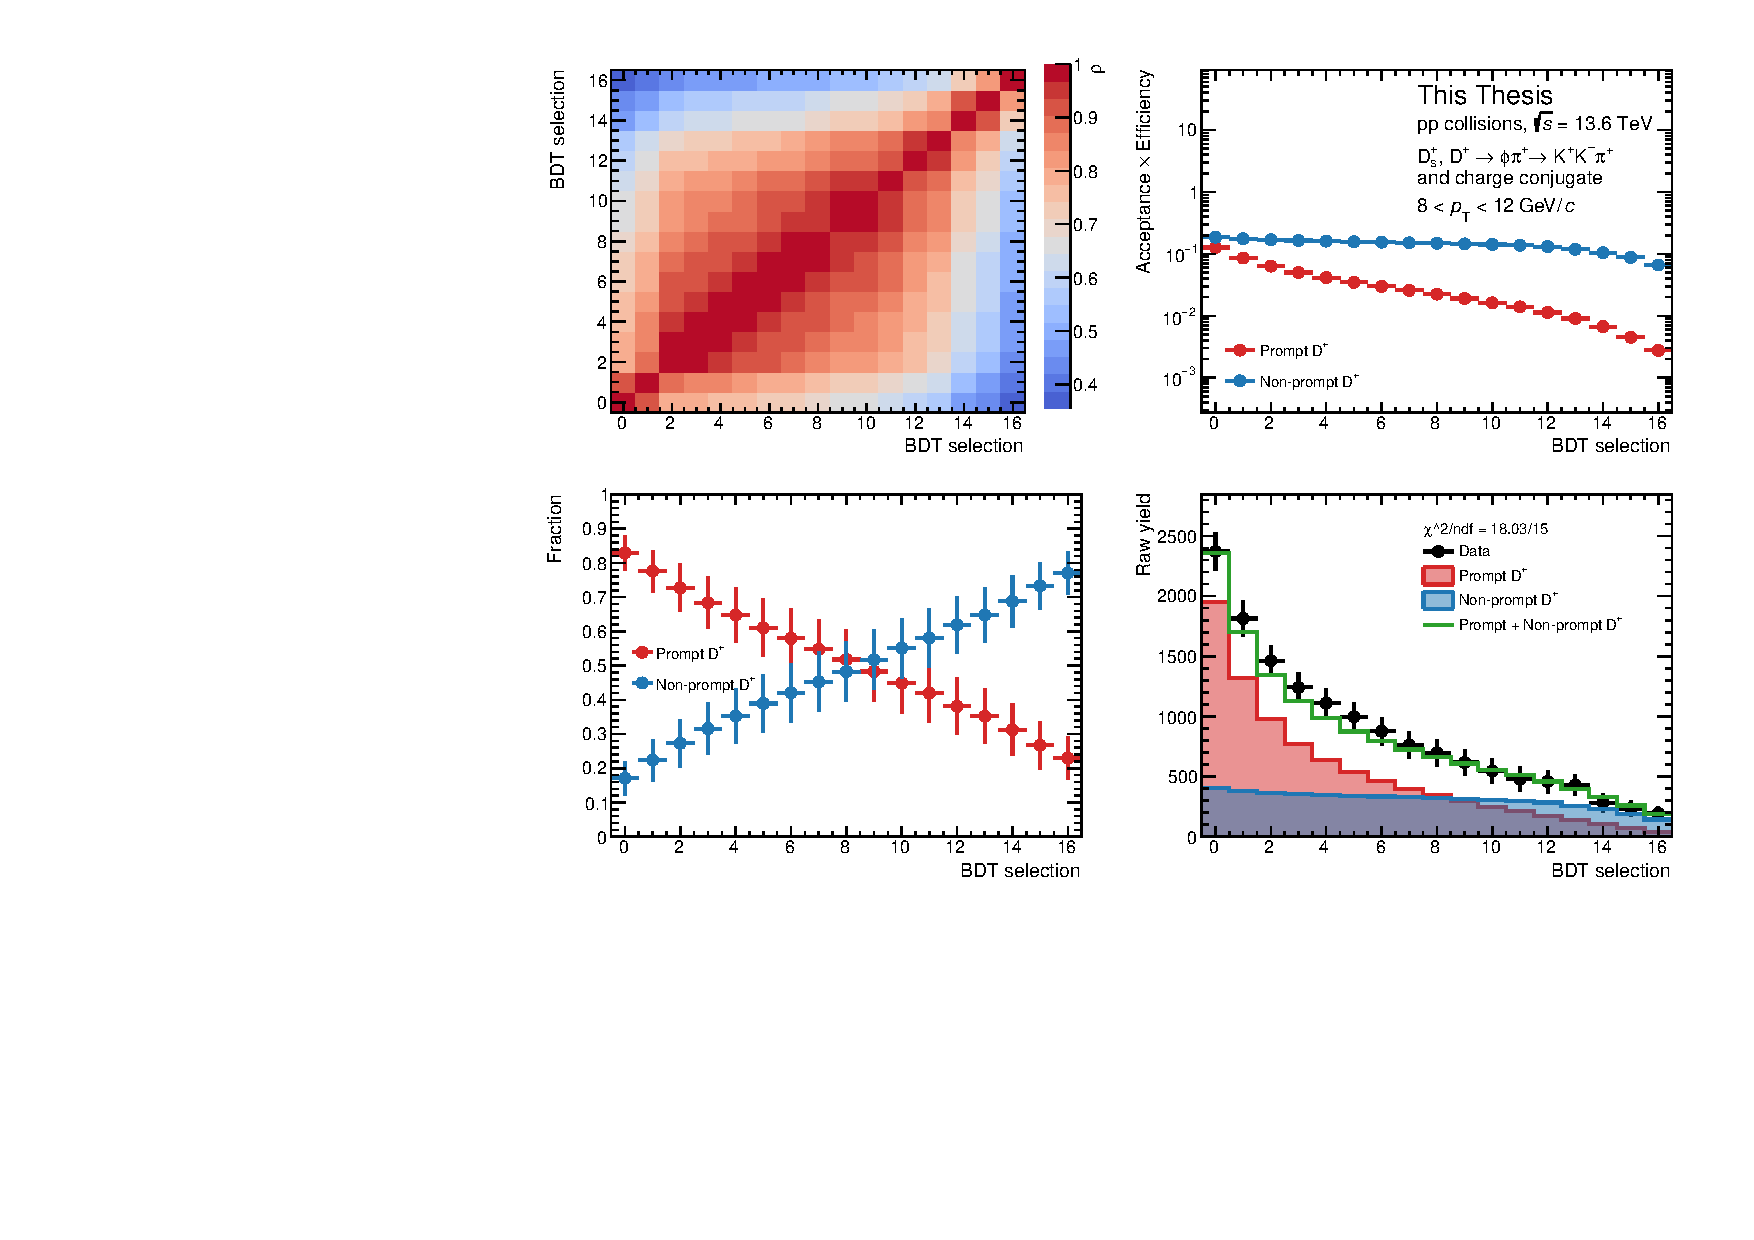
\includegraphics[width=0.7\textwidth]{Figures/Chapter 6/AllPropmtFracs/Dplus/DplusPromptFrac80_120.pdf}
    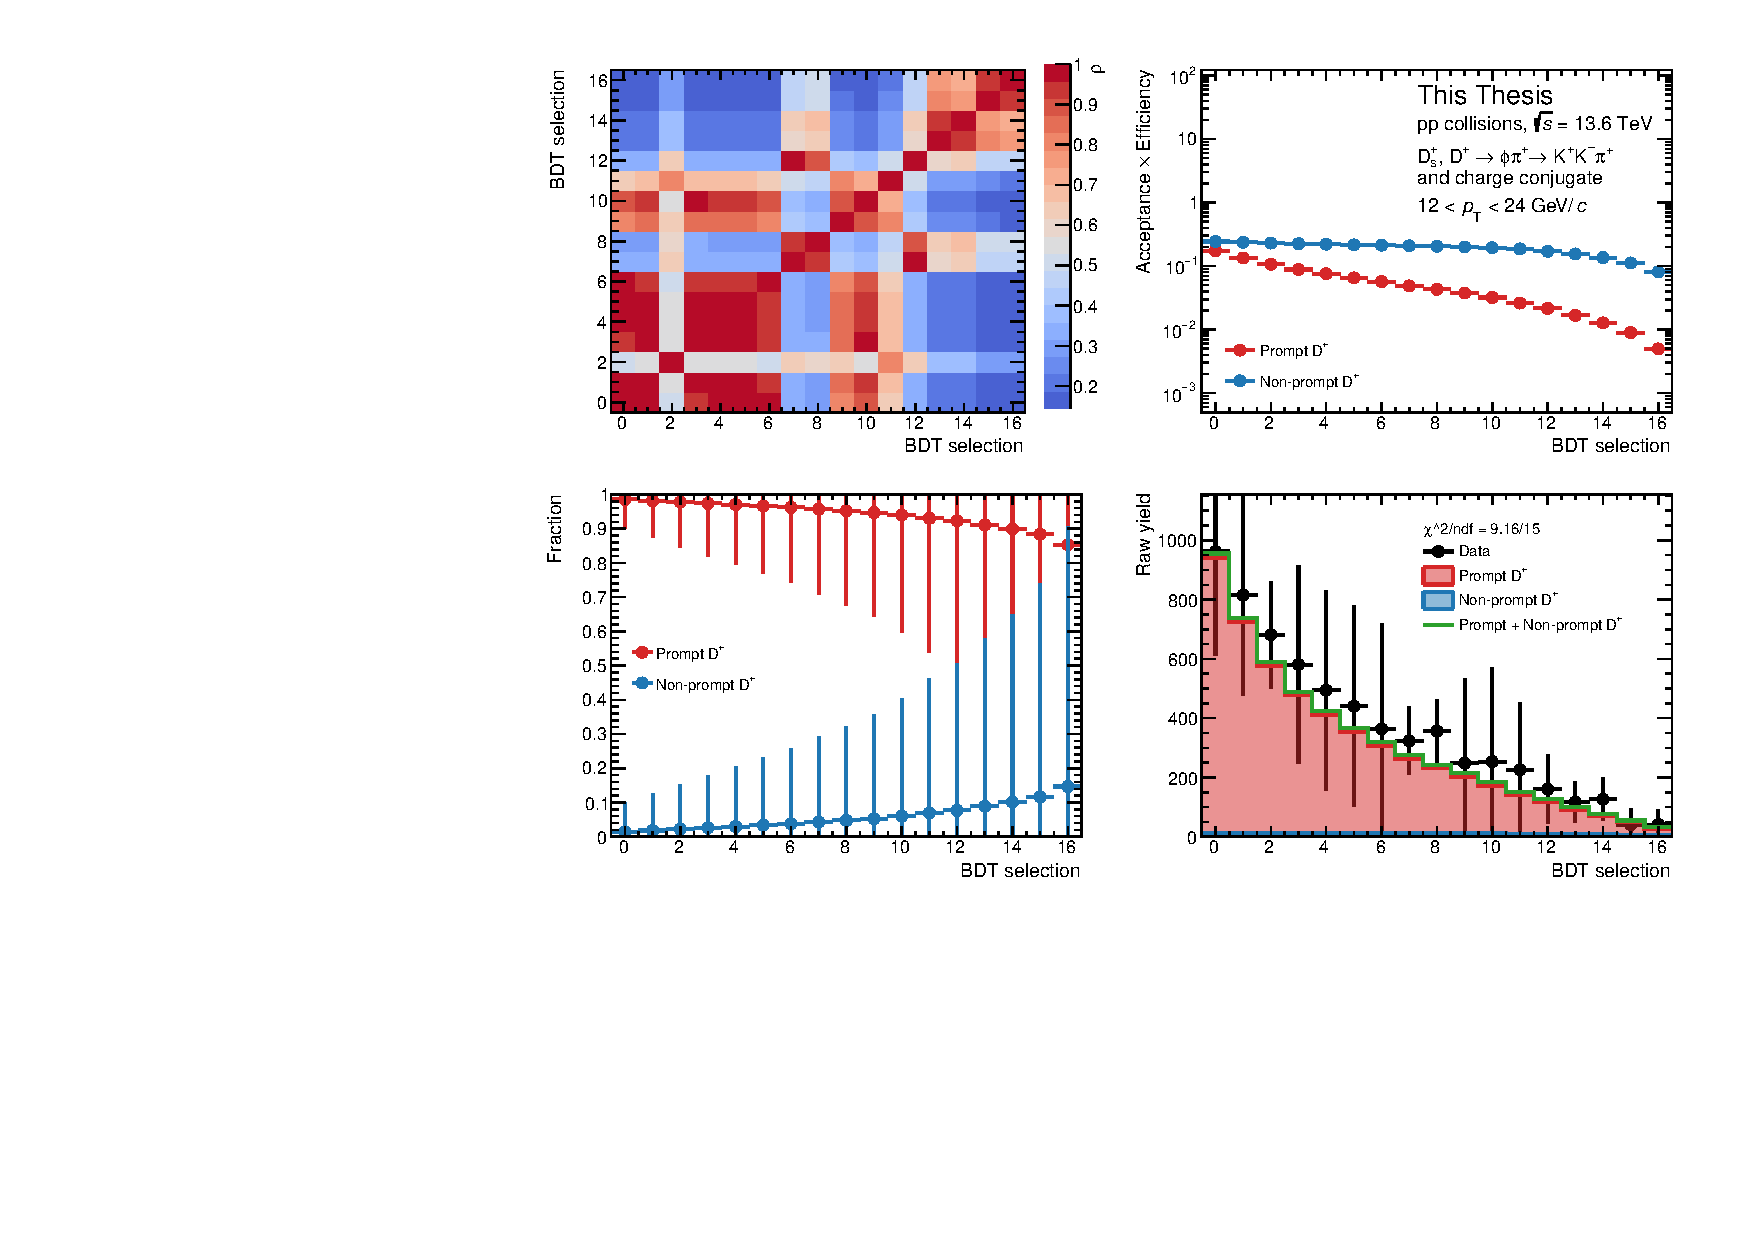
\includegraphics[width=0.7\textwidth]{Figures/Chapter 6/AllPropmtFracs/Dplus/DplusPromptFrac120_240.pdf}
    \caption{Results for the evaluation of the \fpdpl correction factor in the $8.0 < \pt < 12.0$~\gevc (top) and $12.0 < \pt < 24.0$~\gevc (bottom) intervals.}
    \end{figure}
        
